%\usepackage{unicode-math}

\section{Kinematic Fitting}
\label{subsec:KinFit}
Two problems immediately arise in searching for $hh$ events in the $bbWW$ channel: 1) how to correctly identify and match reconstructed jets to the partons from the hard decay, and 2) how to reduce the large $t\bar{t}$ background. Since $t\bar{t}$ is by far the largest background to be considered, any exploitable differences between the $hh$ and $t\bar{t}$ systems can help in addressing both issues. Luckily, there are many different kinematic constraints in either a $t\bar{t}$ or a $hh$ event which can be used to completely reconstruct the event, and more importantly, these constraints differ. A kinematic fitting technique is used to reconstruct candidate events passing basic selection requirements and identify optimal jet assignments by permuting selected jets through each position in a signal hypothesis and calculating a likelihood for each permutation\footnote{ NB:  The analysis was initially optimised with and without kinematic fit, and we demonstrated that kinematic fit helps us gain sensitivity. Due to missing 13 TeV transfer functions, we decided with the EB to drop it for the conf note, but would like to come back to it for the paper. In the interest of documentation, we would like to keep it in the appendix.}.

Multiple kinematic hypotheses can be evaluated for a given event, providing multiple distinct pieces of information. The kinematic constraints involved differ (e.g. three body $m_{T}$ for $t\bar{t}$, two body $m_{h}$ for $hh$) for different hypotheses, and likelihoods can be calculated independently for an event to be $t\bar{t}$-like or $hh$-like. Using a $hh$ hypothesis to select an optimal jet permutation can help to address the first issue of correctly identifying jets from the $hh$ decay, while a $t\bar{t}$ hypothesis can be used to identify and reject events coming from the dominant $t\bar{t}$ background. The mass resolution of measured objects can also be improved if the detector response to reconstructed objects is well known, although this extra information from kinematic fitting is not currently used. In the current analysis, only a $t\bar{t}$ hypothesis is used in order to reject the $t\bar{t}$ background.

The following section details the method behind the kinematic fitting as well as extensions that use information beyond object kinematics in order to produce the final jet assignments. Additionally, a number of different jet-input configurations are studied to determine the optimal method to identify $t\bar{t}$ events. Once identified, these events can be rejected by imposing a cut on the log likelihood of the $t\bar{t}$ hypothesis.

\subsubsection{$t\bar{t}$ Kinematic Fitting} 
The events are reconstructed using a kinematic likelihood code package (KLFitter) \cite{klfitter} which makes use of the Bayesian Analysis Toolkit (BAT) \cite{Caldwell:2008fw}. KLFitter uses an input model (e.g., $hh$, $t\bar{t}$) and mass constraints ($m_{h}$, $m_{T}$, $m_{W}$) on composite objects built from the input leptons, $E_{T}^{miss}$, and jets to map the input particles to leading order partons/leptons from the hard $hh$ or $t\bar{t}$ decay. Transfer functions are used to float the measured energies of the jets and lepton within detector resolutions. Separate transfer functions are defined for jets/leptons/$E_{T}^{miss}$ in different \eta ranges, but the measured angles themselves are assumed to be correctly reconstructed. The final two and three-body masses are evaluated with Breit-Wigner PDFs using (depending on the kinematic hypothesis) $m_{h}$ = 125.0 GeV, $m_{T}$ = 172.5 GeV, and $m_{W}$ = 80.2 GeV. The final expression for the $t\bar{t}$ likelihood, ${L}$, is then expressed as 

%\iffalse
\begin{eqnarray}
&& \mathcal{L}=BW(m_{q_1q_2q_3}| m_{T}\Gamma_{t})\cdot BW(m_{q_1q_2}| m_{W}\Gamma_{W})\cdot BW(m_{q_4\ell\nu}| m_{T}\Gamma_{t})\cdot BW(m_{\ell\nu} | m_{W}\Gamma_{W}) \nonumber \\
&& \prod\limits_{i=1}^4 W_{jet}(E_{i}^{meas}|E_{i})\cdot W_{\ell}(E_{\ell}^{meas}|E_{\ell})\cdot W_{miss}(E_{x}^{miss}|p_{x}^{\nu})\cdot W_{miss}(E_{y}^{miss}|p_{y}^{\nu}) .
\label{eq:KLF}
\end{eqnarray}
%\fi

where $W_{i}(E_{x}^{meas}|E_{i})$ are the transfer functions, $E_{x}^{meas}$ is the measured energy of object $x$, $E_{i}$ is the 'true' energy of the reconstructed parton $i$, and the $BW(m_{ij(k)}| m_{Y}\Gamma_{Y})$ are the Breit-Wigner functions used to evaluate the mass of composite reconstructed particles with respect to a set mass and width of particle $Y$. 

The transfer functions (TF) used in the kinematic fitter are derived for electrons, muons, light jets, b-jets, and $E_{T}^{miss}$ using the $t\bar{t}$ MC sample. As the detector response changes in different regions of the detector and for particles with different energy ranges, a number of transfer functions are defined for each particle species and binned in terms of eta and $p_{T}$. More details about the derivations and kinematics of the transfer functions can be found the KLFitter paper \cite{klfitter}. Validation plots of the KLFitter reconstruction at 8 TeV can be seen in Figure \ref{fig:KLF_validation}.

\begin{figure}[!hb]
\begin{center}
		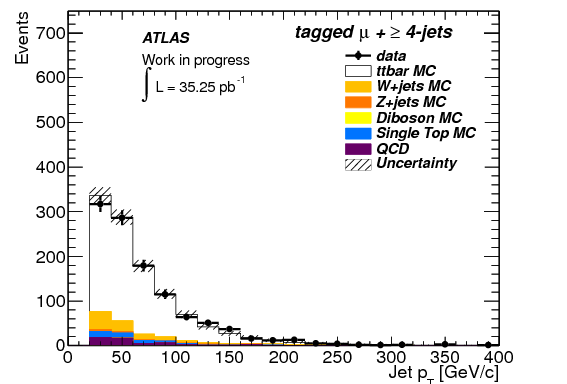
\includegraphics[width=.47\textwidth]{figures/kinFit_appendix/validation/JetpT_mu}
		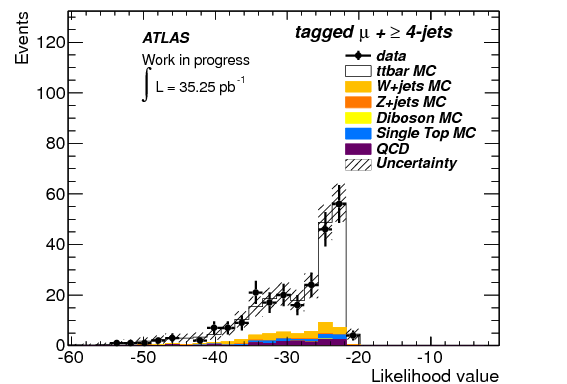
\includegraphics[width=.47\textwidth]{figures/kinFit_appendix/validation/Likelihood_mu}\\
		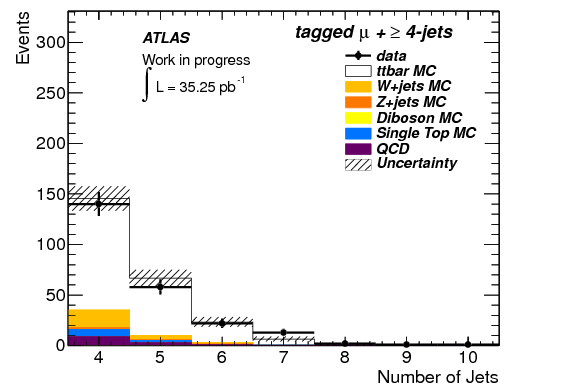
\includegraphics[width=.47\textwidth]{figures/kinFit_appendix/validation/NumberofJets_mu}
		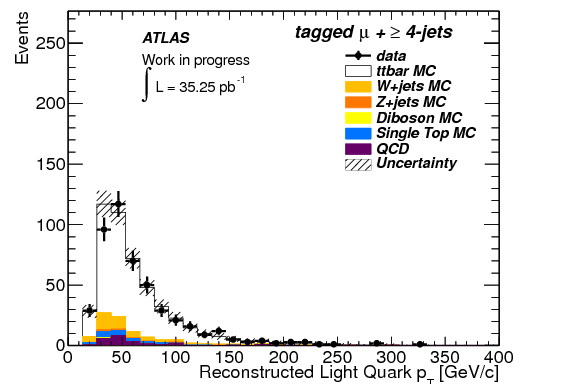
\includegraphics[width=.47\textwidth]{figures/kinFit_appendix/validation/RecoLightQuark_pT_mu}\\
		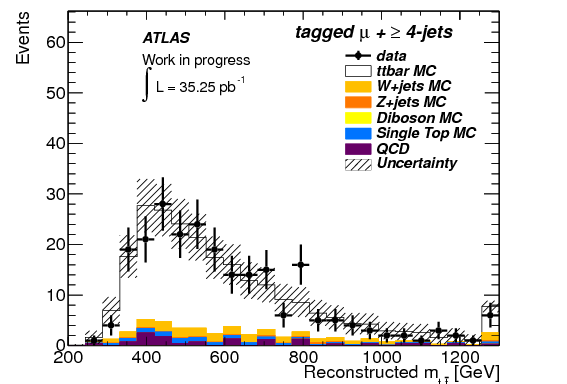
\includegraphics[width=.47\textwidth]{figures/kinFit_appendix/validation/Reco_m_ttbar_mu}
                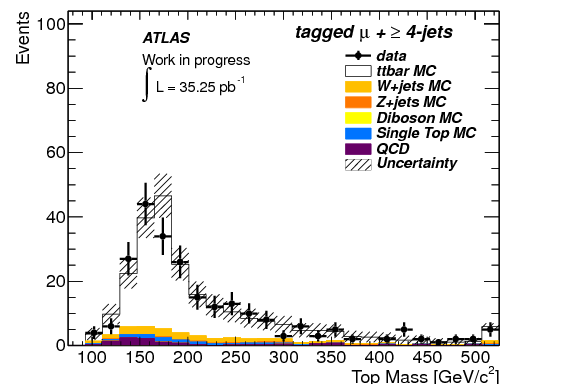
\includegraphics[width=.47\textwidth]{figures/kinFit_appendix/validation/TopMass_mu}
	\caption{Validation plots of KLFitter performance performed at 8 TeV. More can be found in the KLFitter paper~\cite{klfitter}.}
	\label{fig:KLF_validation}
	\end{center}    
	\end{figure}

Permuting the jets in an event through all positions in the model hypothesis yields different values for each permutation using Eq. \ref{eq:KLF}. After the likelihood of each permutation is calculated, the results are ordered, and the best permutation (defined as the permutation with the highest og likelihood) is used to assign jets and optimize a likelihood cut to reject $t\bar{t}$ events. Reconstructed distributions from the leading permutation are shown in Figures \ref{fig:klfitter_control_plots_bbpt150}, Figures \ref{fig:klfitter_control_plots_bbpt150_nf1168}, \ref{fig:klfitter_control_plots_bbpt350}, and \ref{fig:klfitter_control_plots_bbpt350_nf1190}. Decent agreement between data and prediction is observed in all signal regions.

\begin{figure}[!hb]
\begin{center}
		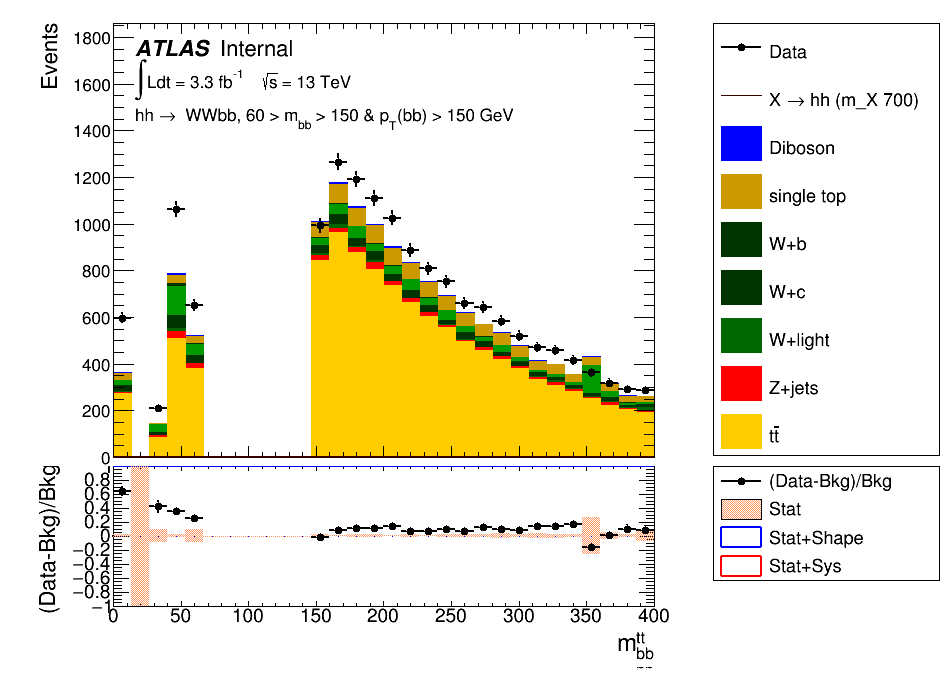
\includegraphics[width=.47\textwidth]{figures/kinFit_appendix/bbpt150/C_mBBcr_opt700_bbpt150_KLF_ttbar_bb_m}
		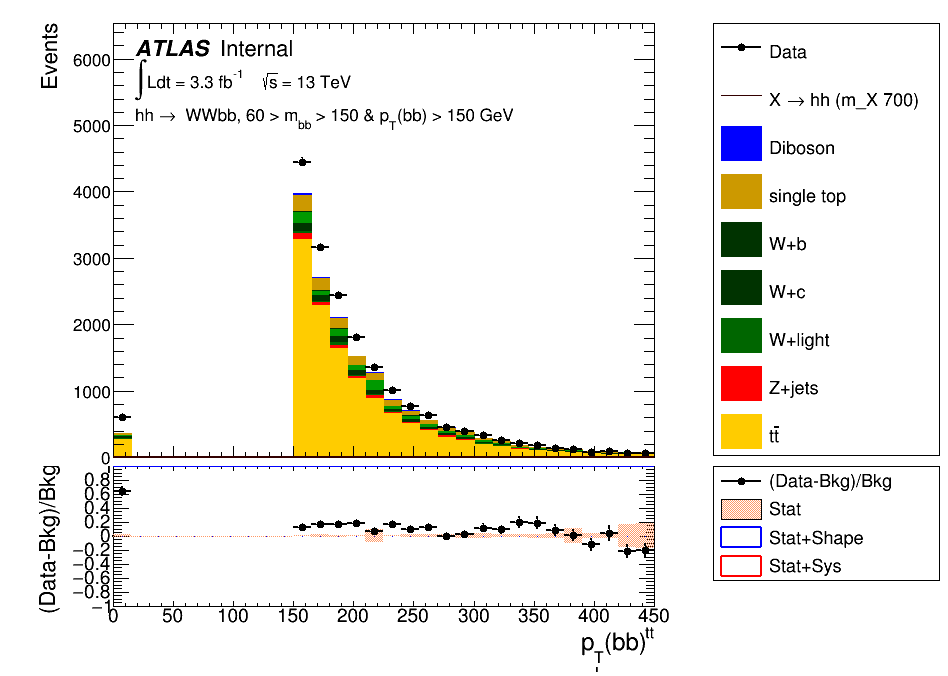
\includegraphics[width=.47\textwidth]{figures/kinFit_appendix/bbpt150/C_mBBcr_opt700_bbpt150_KLF_ttbar_bb_pt}\\
		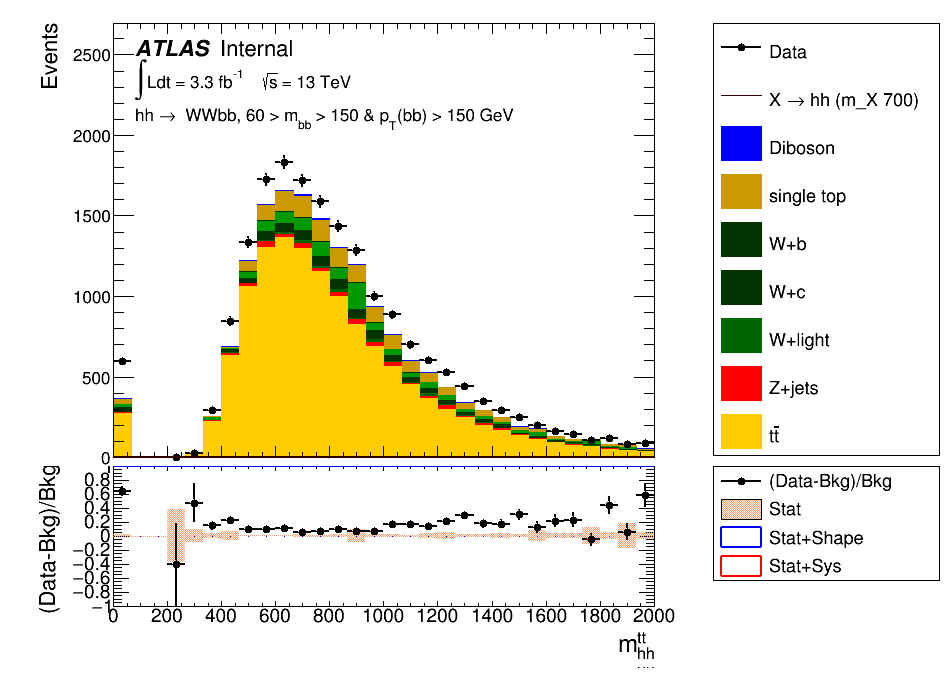
\includegraphics[width=.47\textwidth]{figures/kinFit_appendix/bbpt150/C_mBBcr_opt700_bbpt150_KLF_ttbar_hh_m}
		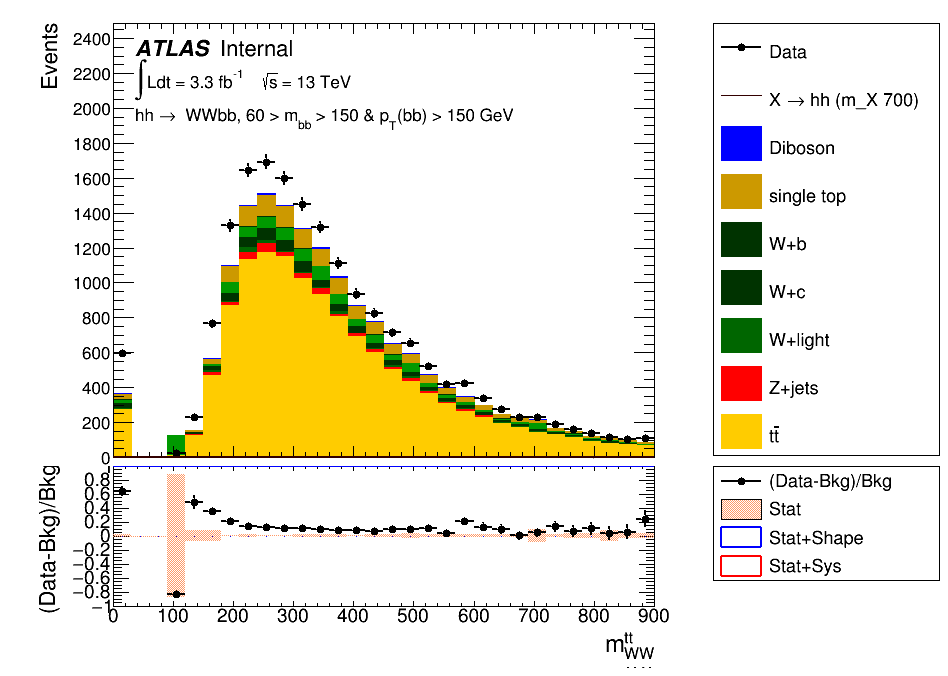
\includegraphics[width=.47\textwidth]{figures/kinFit_appendix/bbpt150/C_mBBcr_opt700_bbpt150_KLF_ttbar_ww_m}\\
		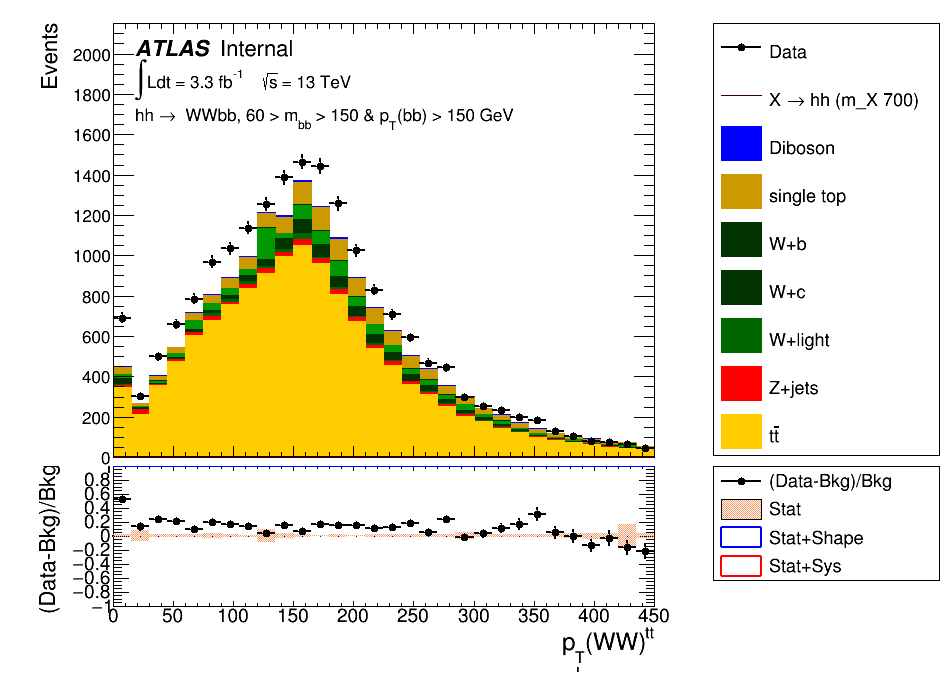
\includegraphics[width=.47\textwidth]{figures/kinFit_appendix/bbpt150/C_mBBcr_opt700_bbpt150_KLF_ttbar_ww_pt}
                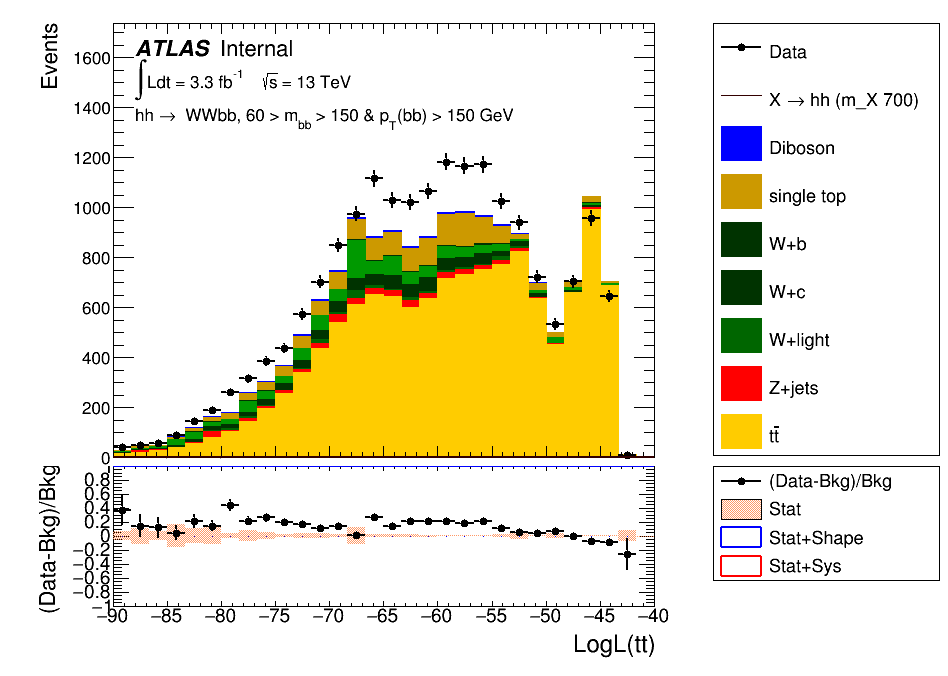
\includegraphics[width=.47\textwidth]{figures/kinFit_appendix/bbpt150/C_mBBcr_opt700_bbpt150_LogLikelihood_ttbar}
	\caption{These control plots show data/prediction agreement using the \ttbar kinematic fitting hypothesis in CR1 for select measured kinematics and the log likelihood of the leading permutation (ranked by event probability).}
	\label{fig:klfitter_control_plots_bbpt150}
	\end{center}    
	\end{figure}


\begin{figure}[!hb]
\begin{center}
		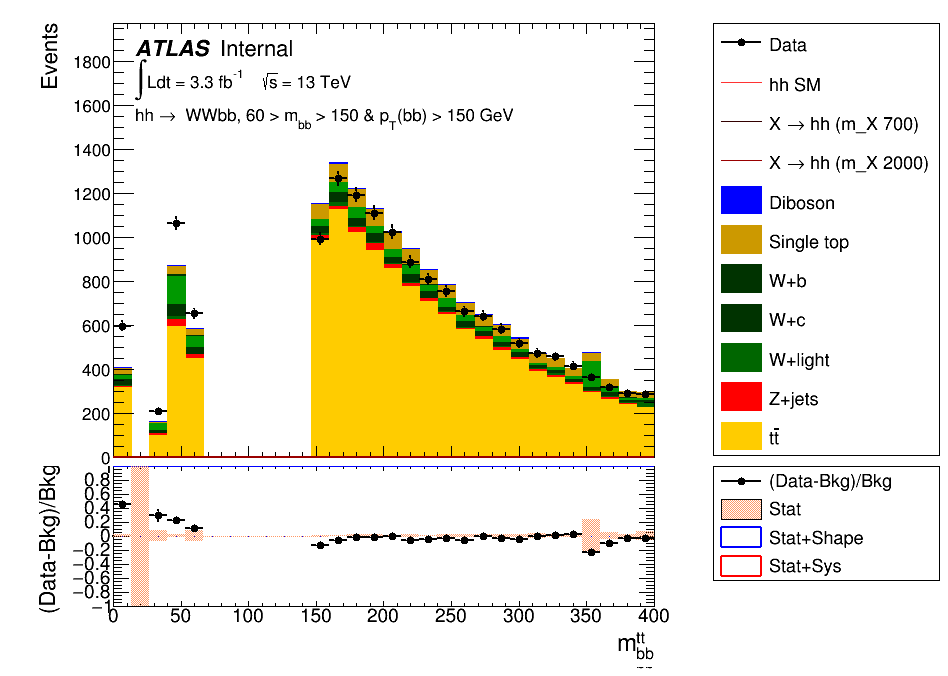
\includegraphics[width=.47\textwidth]{figures/kinFit_appendix/bbpt150_NF1168/C_mBBcr_opt700_bbpt150_KLF_ttbar_bb_m}
		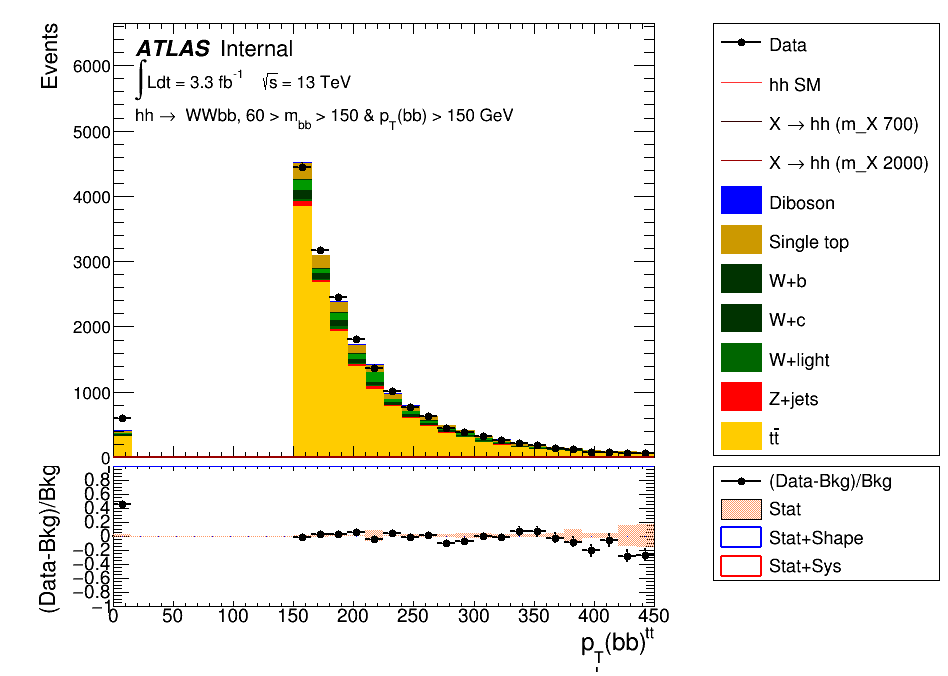
\includegraphics[width=.47\textwidth]{figures/kinFit_appendix/bbpt150_NF1168/C_mBBcr_opt700_bbpt150_KLF_ttbar_bb_pt}\\
		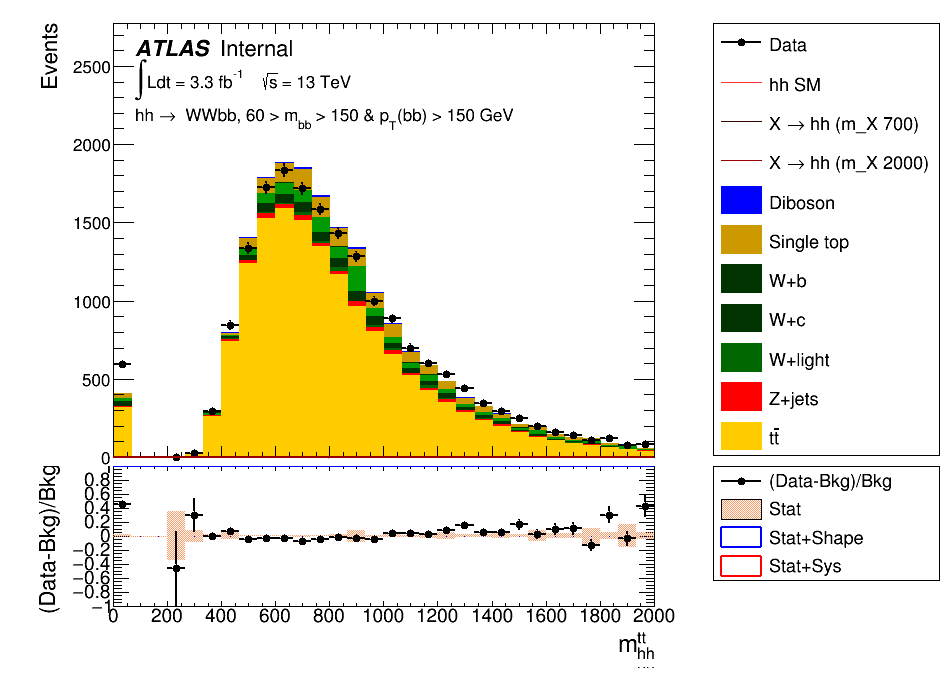
\includegraphics[width=.47\textwidth]{figures/kinFit_appendix/bbpt150_NF1168/C_mBBcr_opt700_bbpt150_KLF_ttbar_hh_m}
		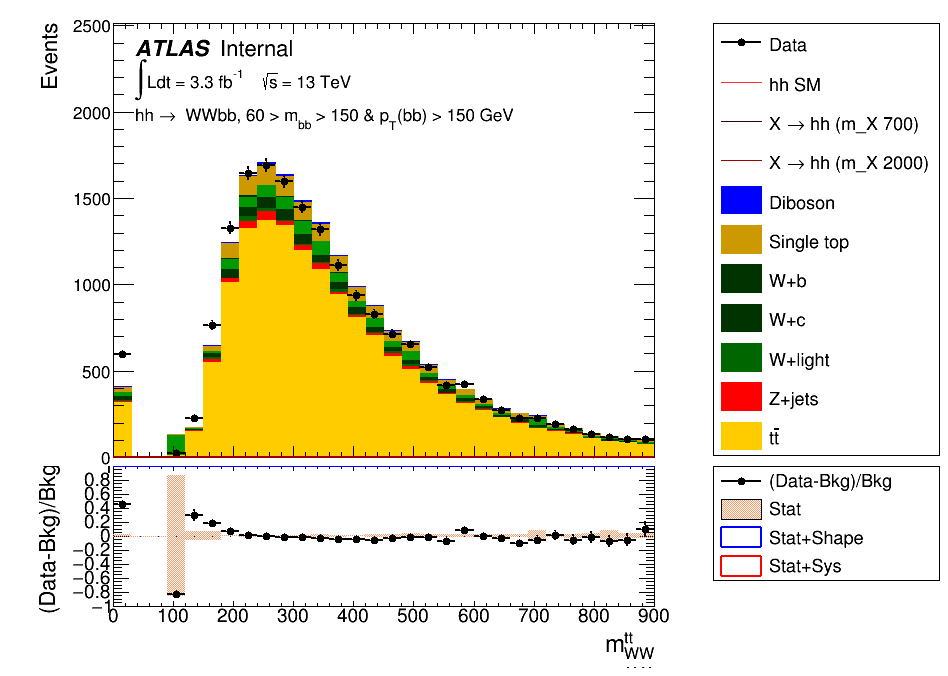
\includegraphics[width=.47\textwidth]{figures/kinFit_appendix/bbpt150_NF1168/C_mBBcr_opt700_bbpt150_KLF_ttbar_ww_m}\\
		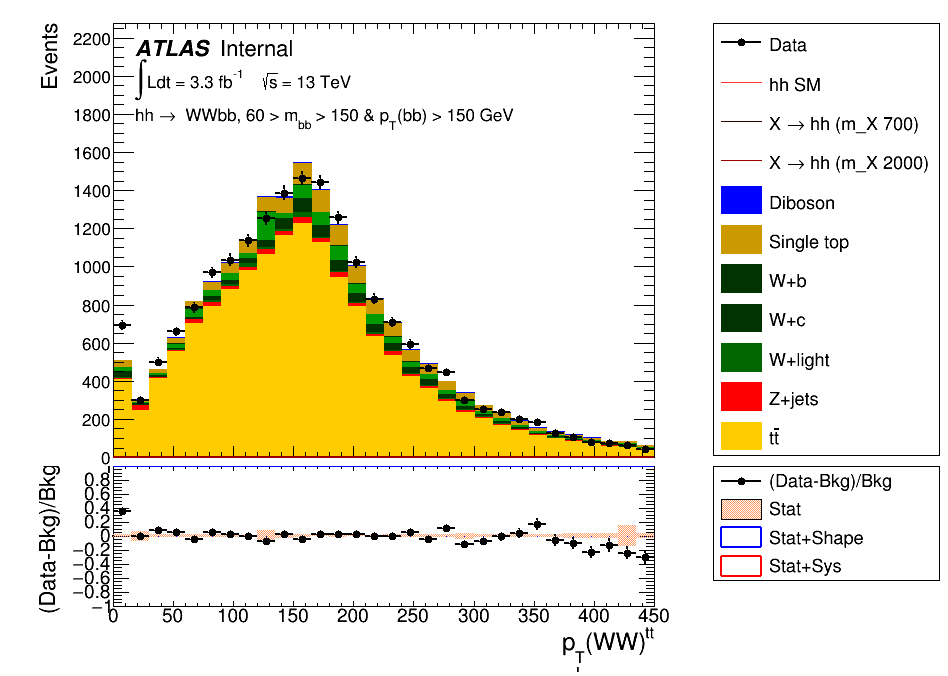
\includegraphics[width=.47\textwidth]{figures/kinFit_appendix/bbpt150_NF1168/C_mBBcr_opt700_bbpt150_KLF_ttbar_ww_pt}
                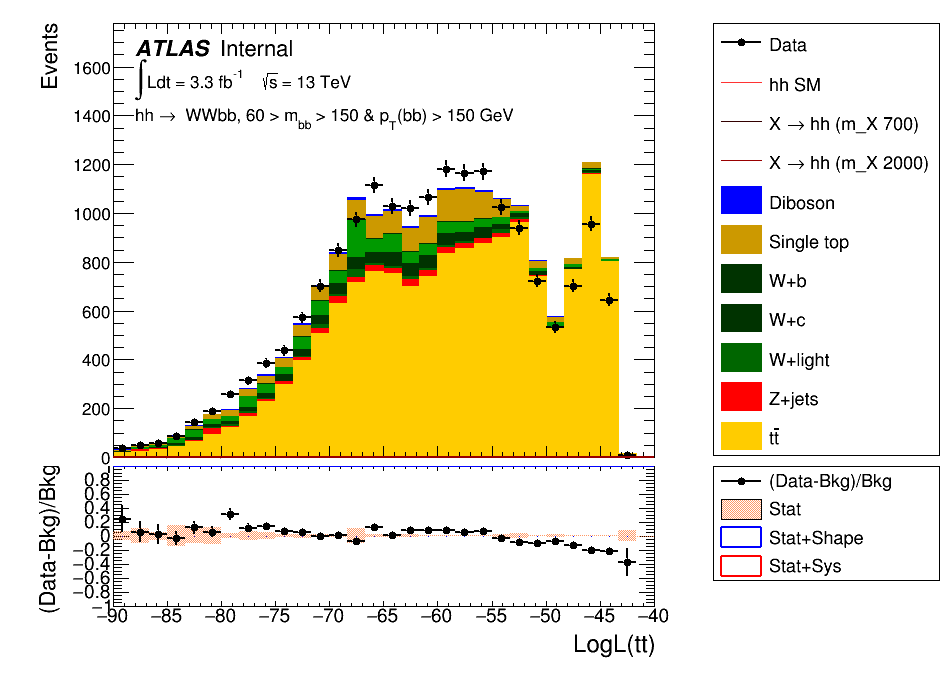
\includegraphics[width=.47\textwidth]{figures/kinFit_appendix/bbpt150_NF1168/C_mBBcr_opt700_bbpt150_LogLikelihood_ttbar}
	\caption{These control plots show data/prediction agreement using the \ttbar kinematic fitting hypothesis in CR1 for select measured kinematics and the log likelihood of the leading permutation (ranked by event probability) after normalising $t\bar{t}$ as described in Sec~\ref{subsec:topCR}.}
	\label{fig:klfitter_control_plots_bbpt150_nf1168}
	\end{center}    
	\end{figure}


\begin{figure}[!hb]
\begin{center}
		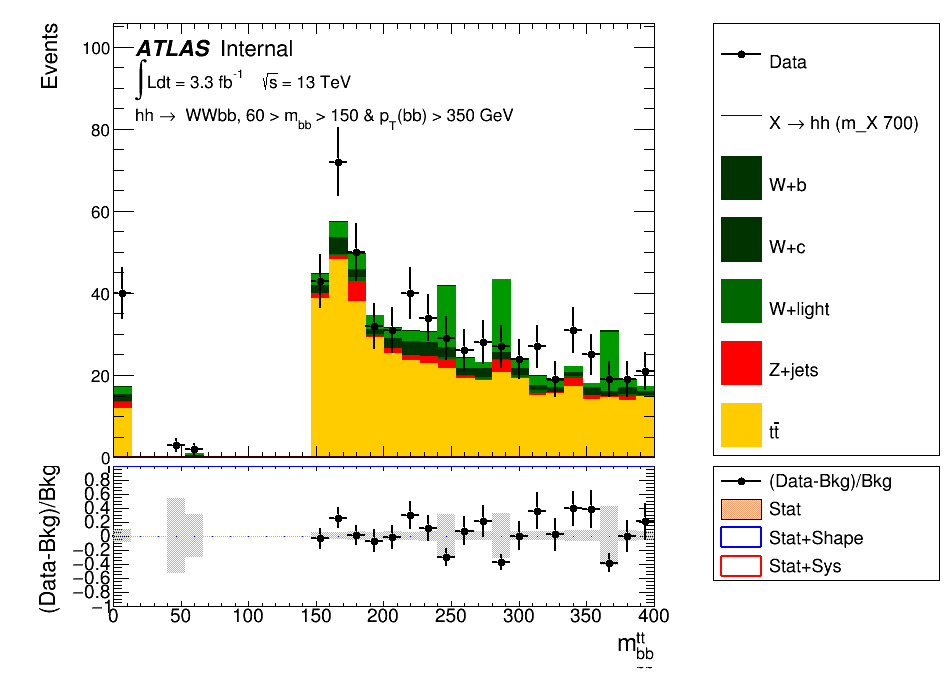
\includegraphics[width=.47\textwidth]{figures/kinFit_appendix/bbpt350/C_mBBcr_opt2000_bbpt350_KLF_ttbar_bb_m}
		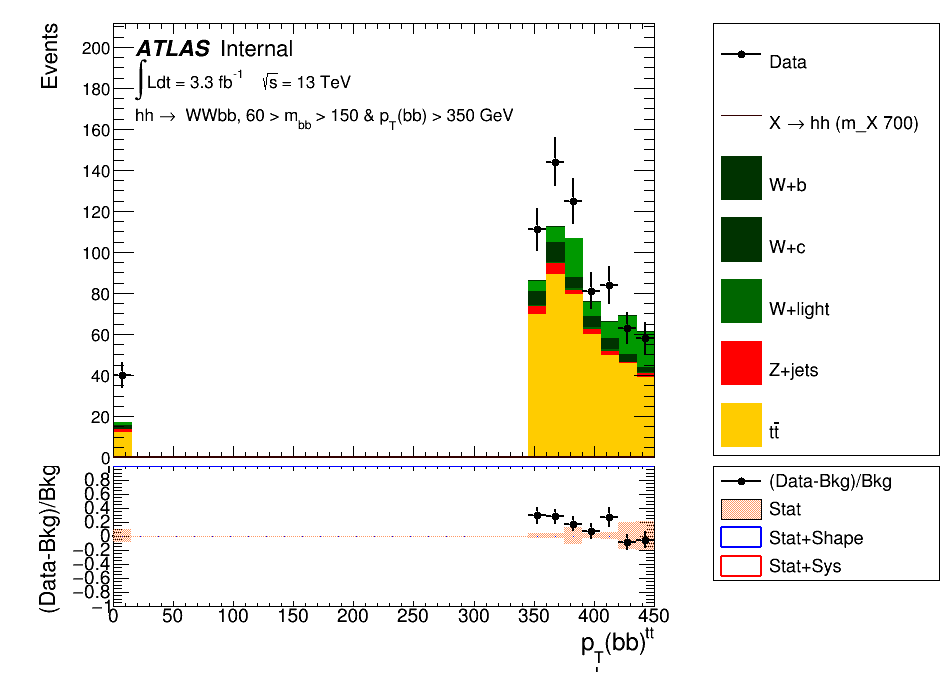
\includegraphics[width=.47\textwidth]{figures/kinFit_appendix/bbpt350/C_mBBcr_opt2000_bbpt350_KLF_ttbar_bb_pt}\\
		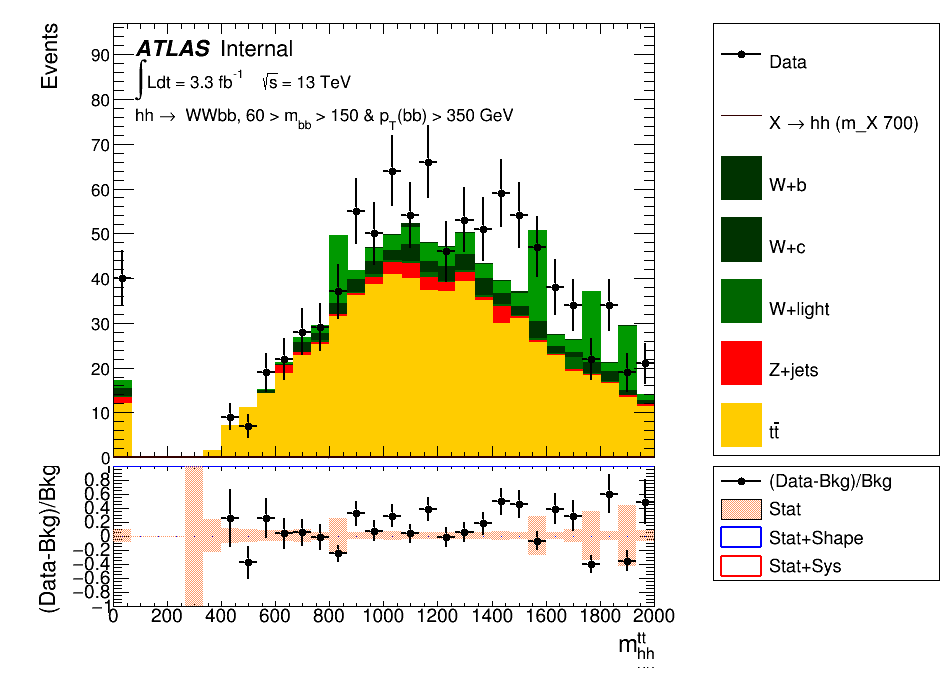
\includegraphics[width=.47\textwidth]{figures/kinFit_appendix/bbpt350/C_mBBcr_opt2000_bbpt350_KLF_ttbar_hh_m}
		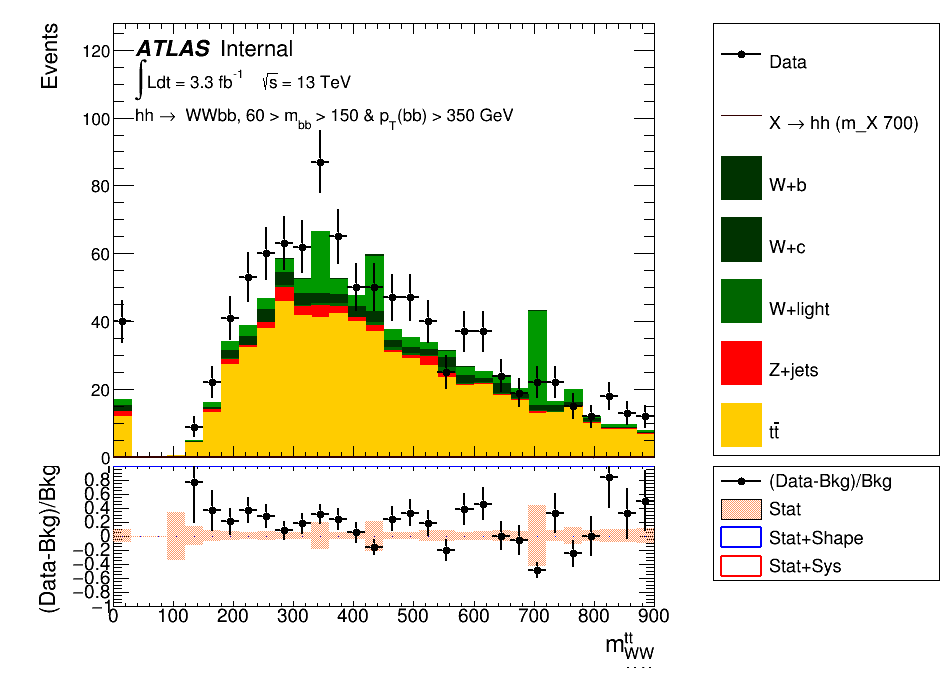
\includegraphics[width=.47\textwidth]{figures/kinFit_appendix/bbpt350/C_mBBcr_opt2000_bbpt350_KLF_ttbar_ww_m}\\
		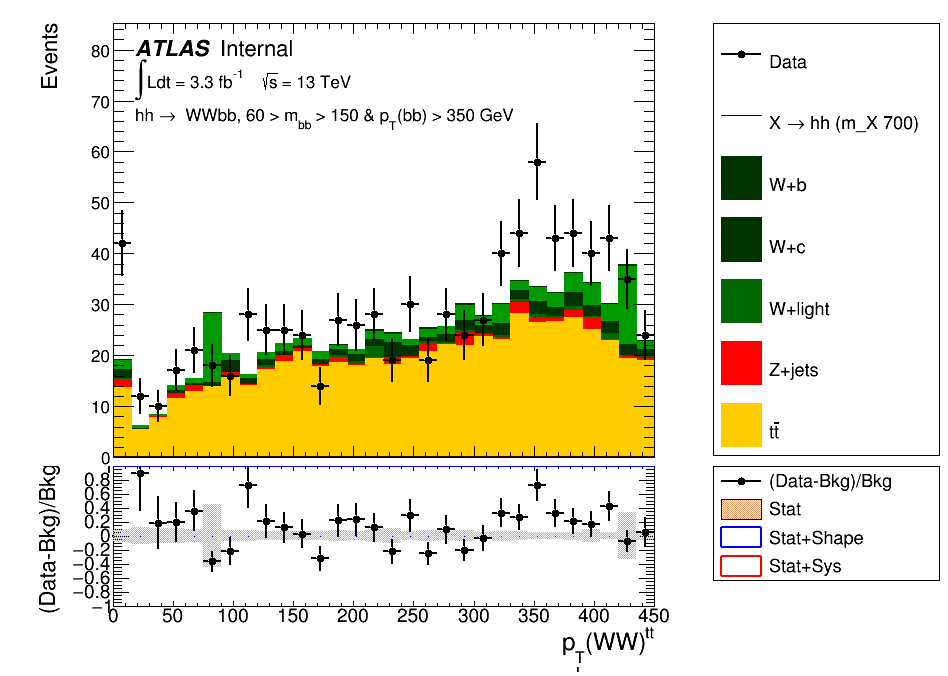
\includegraphics[width=.47\textwidth]{figures/kinFit_appendix/bbpt350/C_mBBcr_opt2000_bbpt350_KLF_ttbar_ww_pt}
                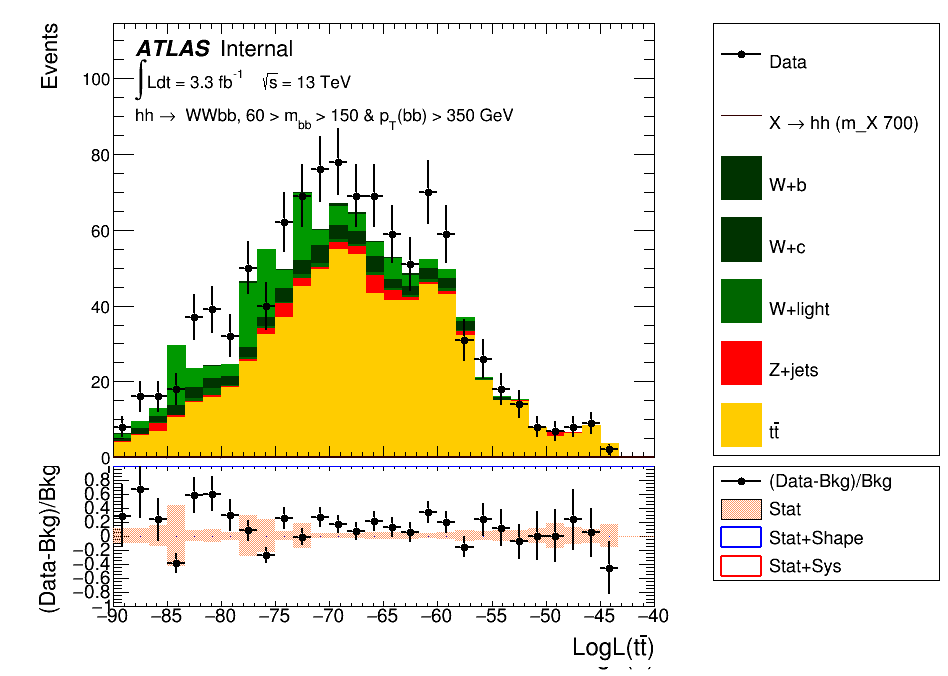
\includegraphics[width=.47\textwidth]{figures/kinFit_appendix/bbpt350/C_mBBcr_opt2000_bbpt350_LogLikelihood_ttbar}
	\caption{These control plots show data/prediction agreement using the \ttbar kinematic fitting hypothesis in CR2 for select measured kinematics and the log likelihood of the leading permutation (ranked by event probability).}
	\label{fig:klfitter_control_plots_bbpt350}
	\end{center}    
	\end{figure}


\begin{figure}[!hb]
\begin{center}
		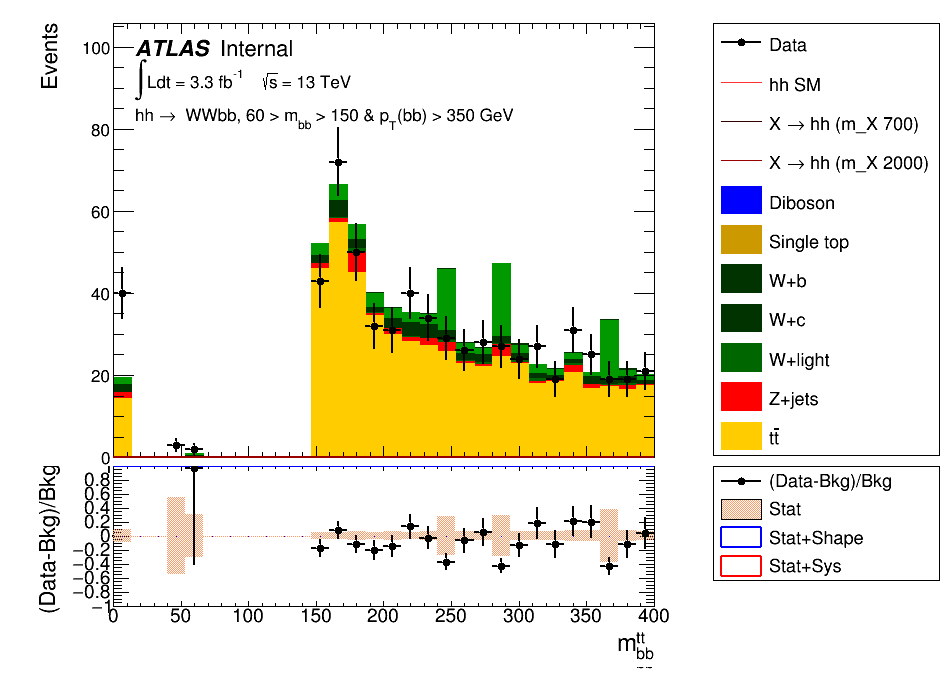
\includegraphics[width=.47\textwidth]{figures/kinFit_appendix/bbpt350_NF1190/C_mBBcr_opt2000_bbpt350_KLF_ttbar_bb_m}
		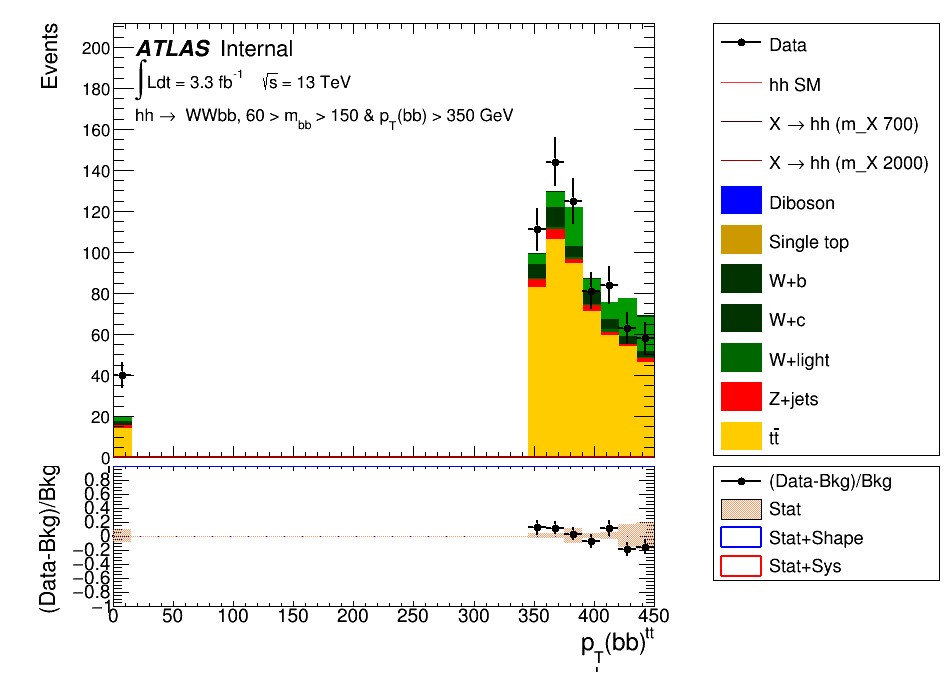
\includegraphics[width=.47\textwidth]{figures/kinFit_appendix/bbpt350_NF1190/C_mBBcr_opt2000_bbpt350_KLF_ttbar_bb_pt}\\
		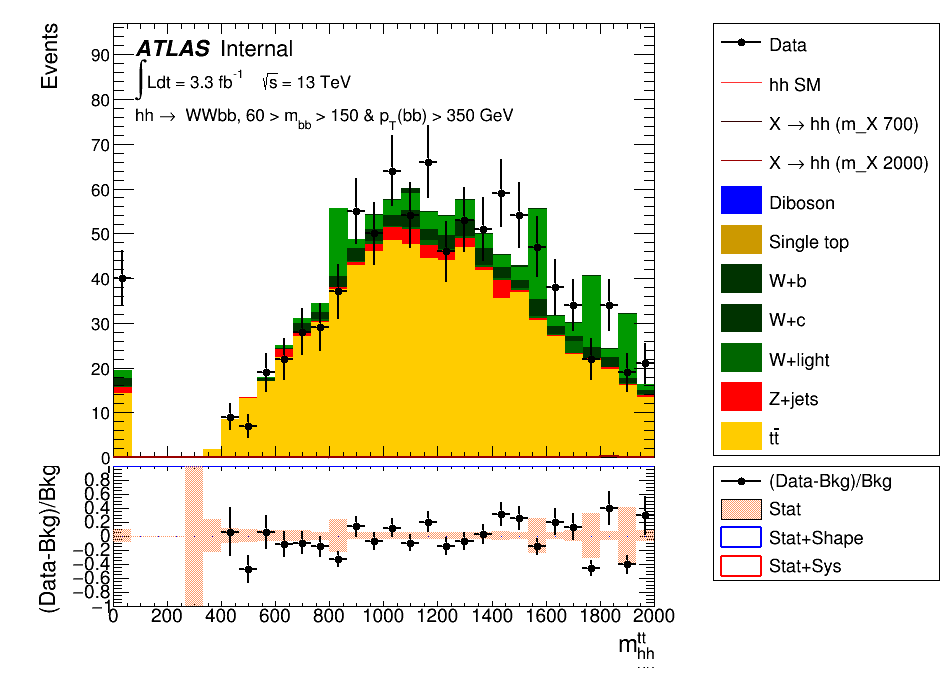
\includegraphics[width=.47\textwidth]{figures/kinFit_appendix/bbpt350_NF1190/C_mBBcr_opt2000_bbpt350_KLF_ttbar_hh_m}
		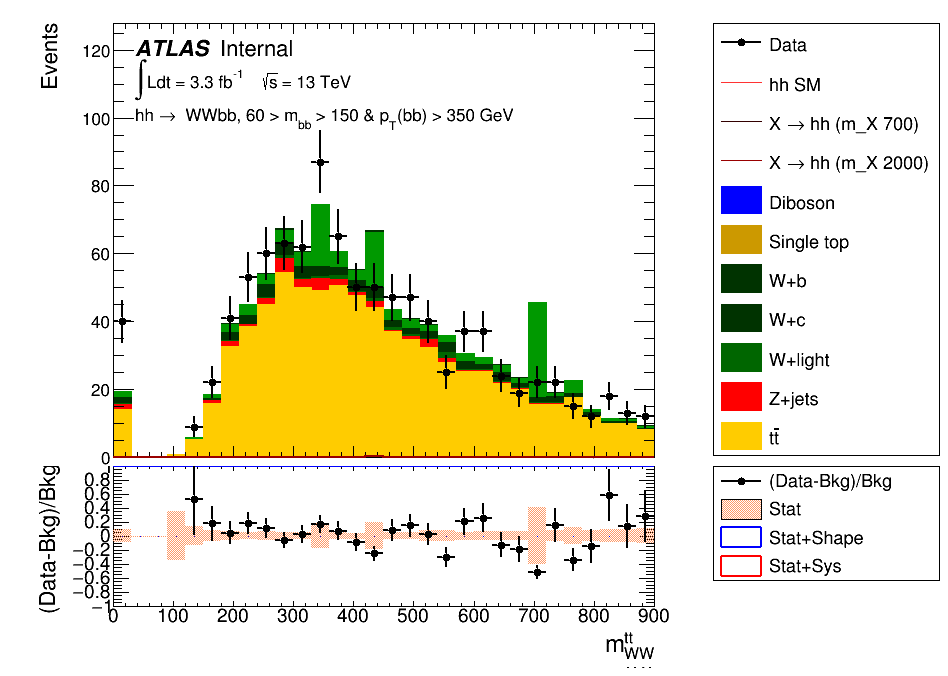
\includegraphics[width=.47\textwidth]{figures/kinFit_appendix/bbpt350_NF1190/C_mBBcr_opt2000_bbpt350_KLF_ttbar_ww_m}\\
		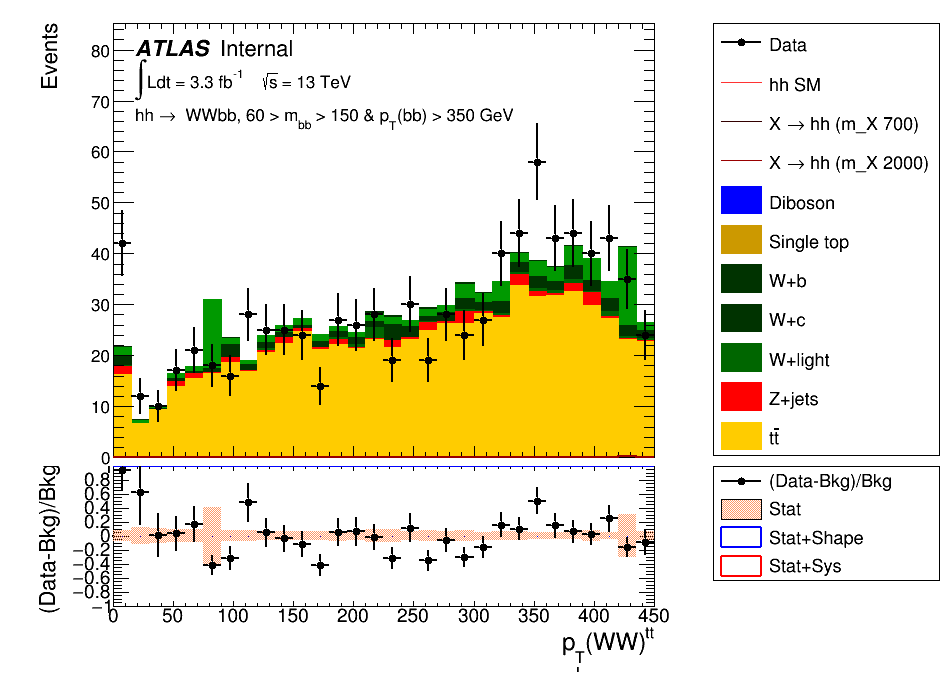
\includegraphics[width=.47\textwidth]{figures/kinFit_appendix/bbpt350_NF1190/C_mBBcr_opt2000_bbpt350_KLF_ttbar_ww_pt}
                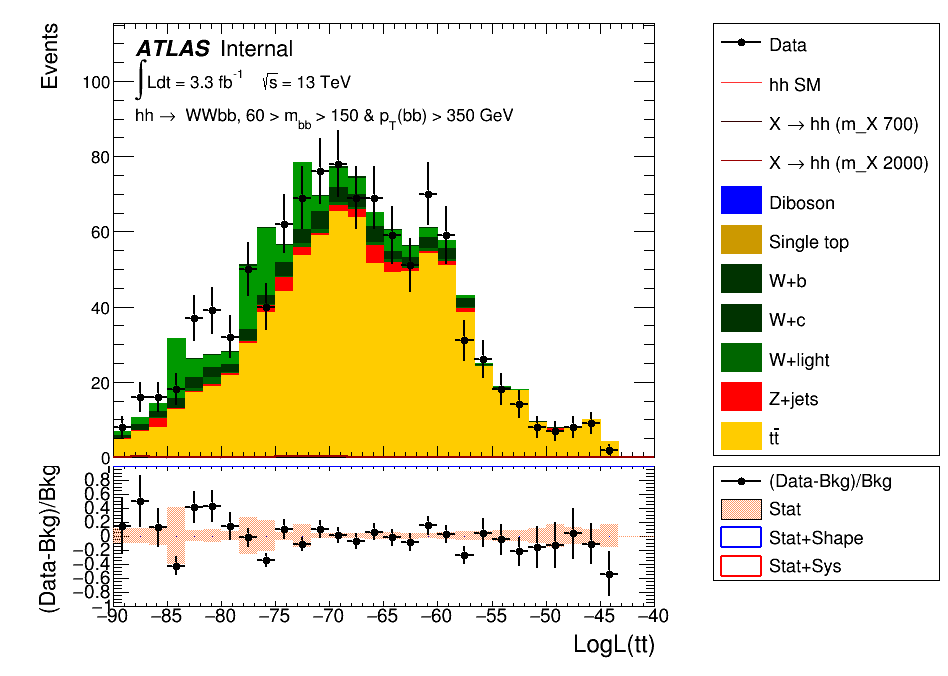
\includegraphics[width=.47\textwidth]{figures/kinFit_appendix/bbpt350_NF1190/C_mBBcr_opt2000_bbpt350_LogLikelihood_ttbar}
	\caption{These control plots show data/prediction agreement using the \ttbar kinematic fitting hypothesis in CR2 for select measured kinematics and the log likelihood of the leading permutation (ranked by event probability) after normalising $t\bar{t}$ as described in Sec~\ref{subsec:topCR}.}
	\label{fig:klfitter_control_plots_bbpt350_nf1190}
	\end{center}    
	\end{figure}	



\subsubsection{Dihiggs Kinematic Fitting} 
An alternative dihiggs kinematic fitting hypothesis can be developed which differs from the \ttbar hypothesis aimed at removing background. For the dihiggs hypothesis, the same jet permuation algorithms and assumptions with respect to the transfer functions, etc. are used, but the invariant masses used to evaluate the permutation are necessarily different. Breit-Wigner PDFs for the $b\bar{b}$ and $WW^*$ higgses are evaluated, and the width is s set to 10 GeV rather than the natural width of the higgs in order to avoid fit failures due to the narrow natural width. Varying the width from 1 to 20 GeV in the likelihood calculation was found to have negligible effect on the final likelihood distribution. No invariant mass requirement on the W's is imposed due to the ambiguity of knowing which W is on-shell. Additionally, no mass constraint is applied on the candidate $hh$ system as the invariant mass constraint is necessarily $X$ resonance dependence. Studies evaluating the efficacy of including these extra constraints are ongoing. The following likelihood is used to evaluate the dihiggs hypothesis


%\iffalse
\begin{eqnarray}
&& \mathcal{L}=BW(m_{q_1q_2}| m_{h}, 10 GeV)\cdot BW(m_{q_3q_4\ell\nu}| m_{h}, 10 GeV) \nonumber \\
&& \prod\limits_{i=1}^4 W_{jet}(E_{i}^{meas}|E_{i})\cdot W_{\ell}(E_{\ell}^{meas}|E_{\ell})\cdot W_{miss}(E_{x}^{miss}|p_{x}^{\nu})\cdot W_{miss}(E_{y}^{miss}|p_{y}^{\nu}) .
\label{eq:KLF}
\end{eqnarray}
%\fi

where, again, $W_{i}(E_{x}^{meas}|E_{i})$ are the transfer functions, $E_{x}^{meas}$ is the measured energy of object $x$, $E_{i}$ is the 'true' energy of the reconstructed parton $i$, and the $BW(m_{ij(k)}| m_{Y}\Gamma_{Y})$ are the Breit-Wigner functions used to evaluate the mass of composite reconstructed particles. Reconstructed distributions from the leading permutation are shown in Figures \ref{fig:klfitter_control_plots_hh_bbpt150_nf1168} and \ref{fig:klfitter_control_plots_hh_bbpt350_nf1190}. Decent agreement between data and prediction is observed in all signal regions.


\begin{figure}[!hb]
\begin{center}
		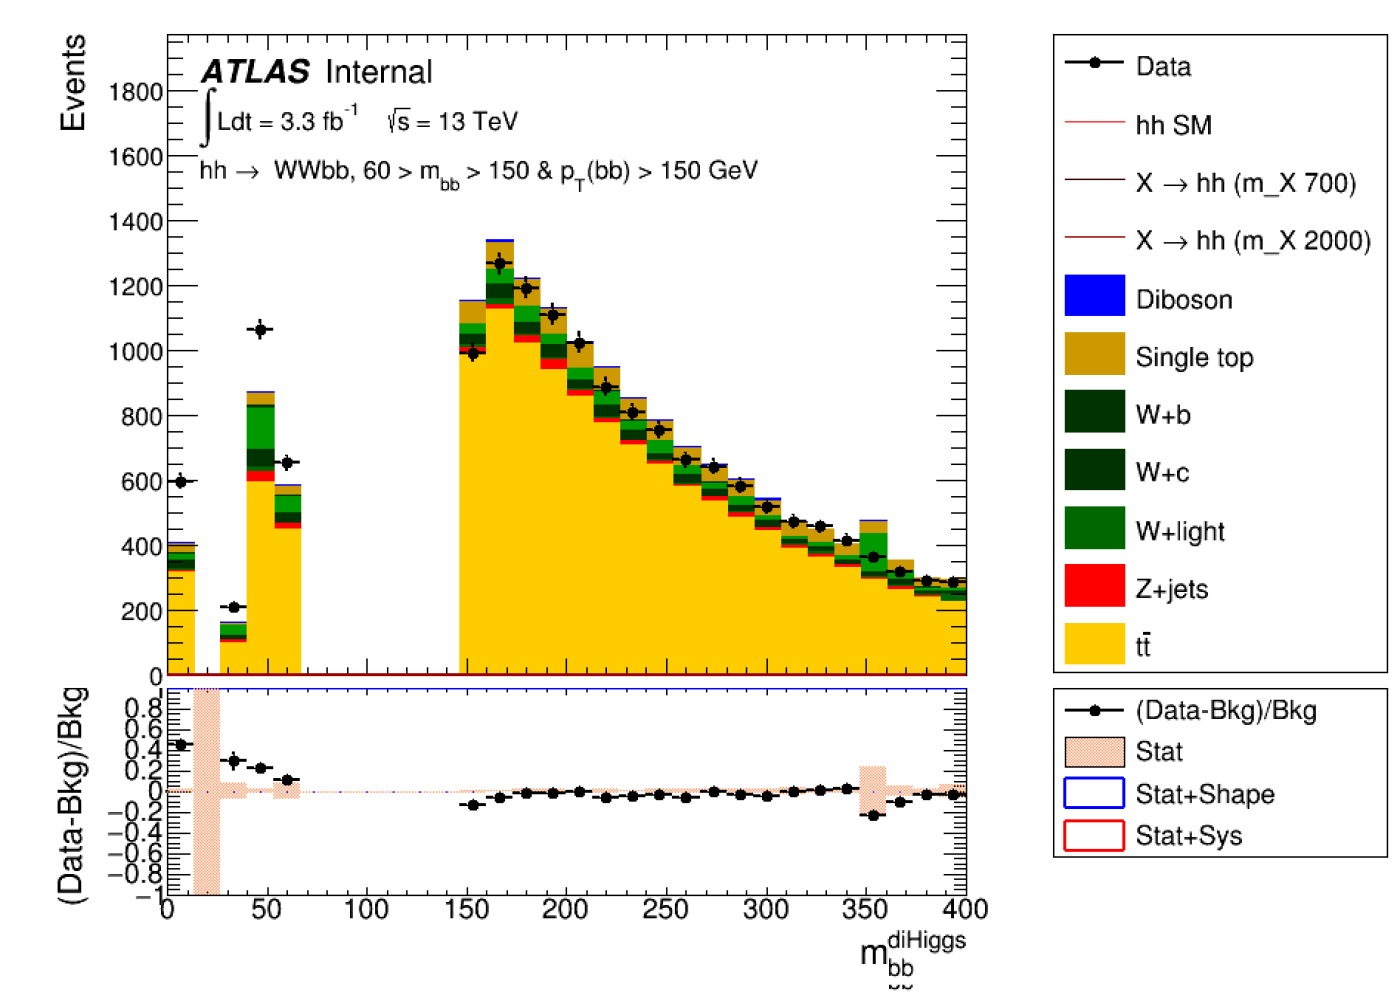
\includegraphics[width=.47\textwidth]{figures/kinFit_appendix/bbpt150_NF1168/C_mBBcr_opt700_bbpt150_KLF_dihiggs_bb_m}
		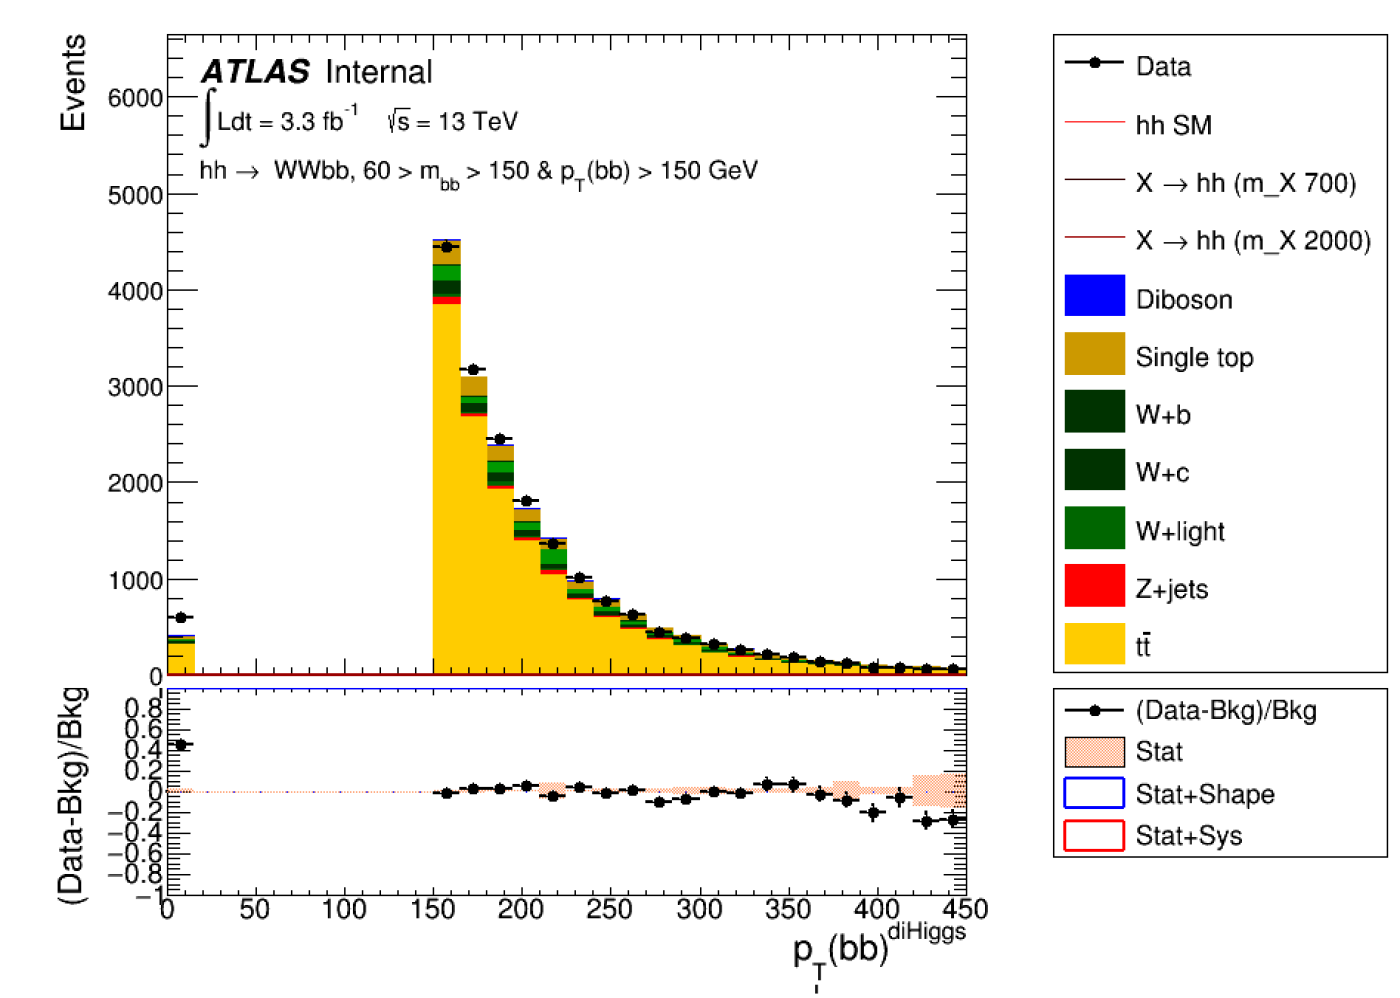
\includegraphics[width=.47\textwidth]{figures/kinFit_appendix/bbpt150_NF1168/C_mBBcr_opt700_bbpt150_KLF_dihiggs_bb_pt}\\
		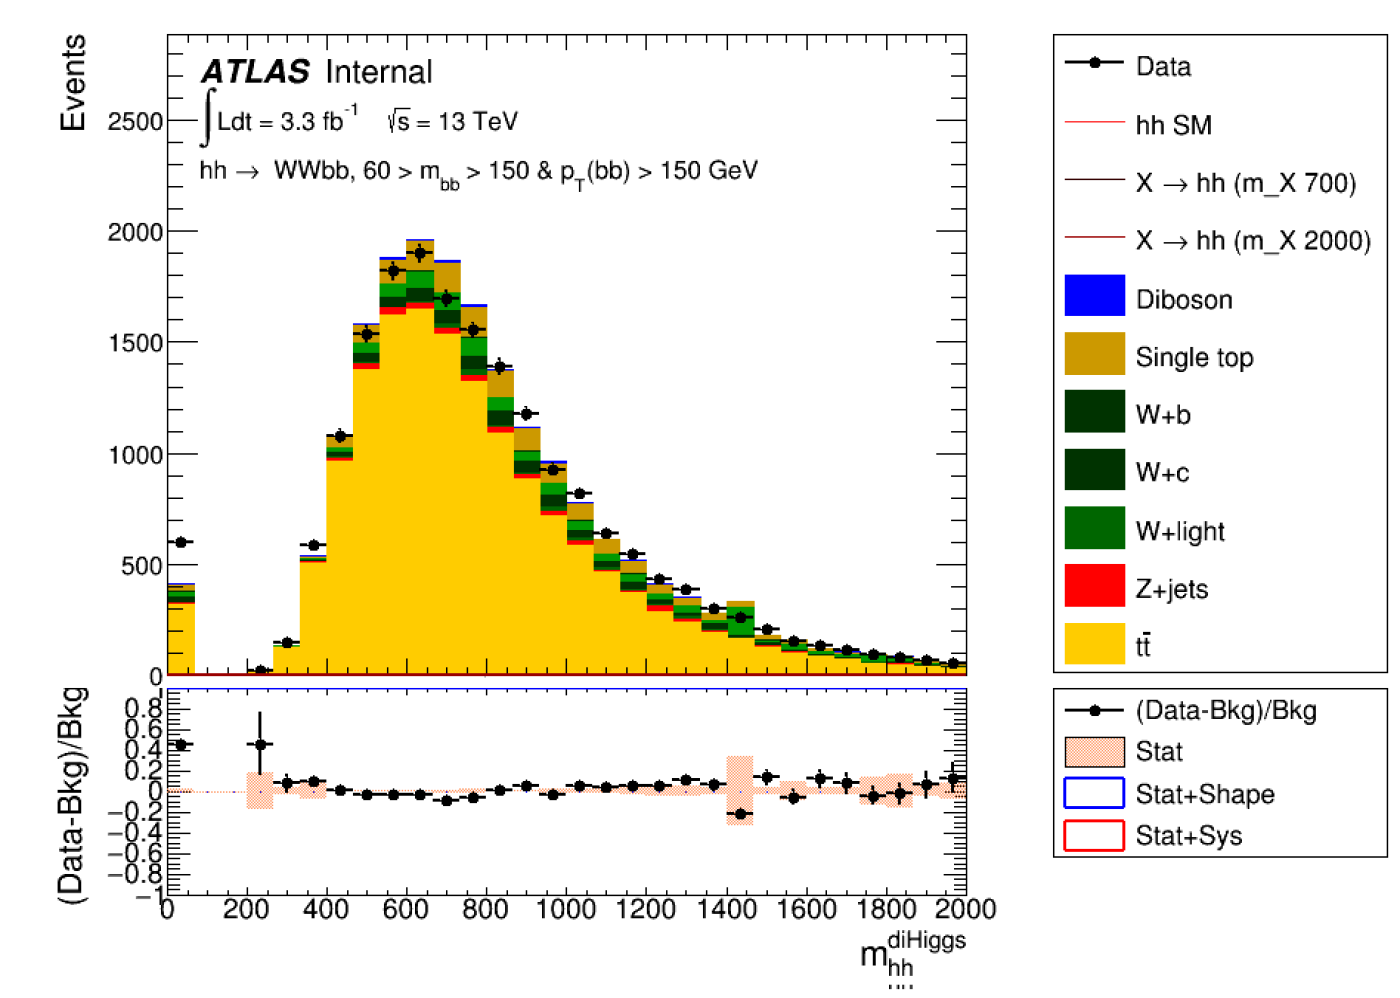
\includegraphics[width=.47\textwidth]{figures/kinFit_appendix/bbpt150_NF1168/C_mBBcr_opt700_bbpt150_KLF_dihiggs_hh_m}
		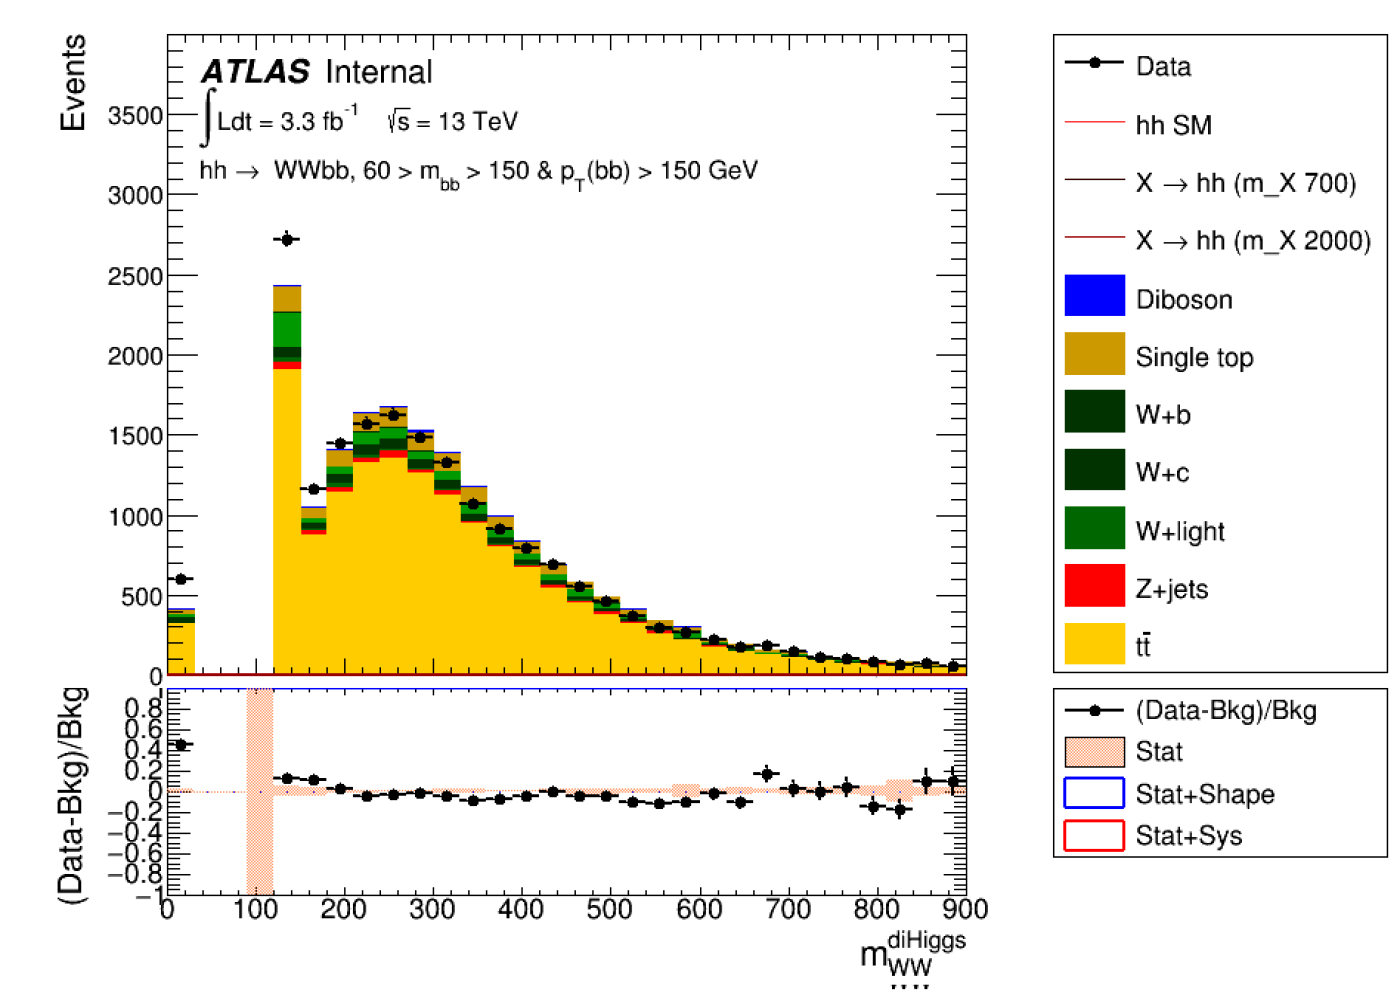
\includegraphics[width=.47\textwidth]{figures/kinFit_appendix/bbpt150_NF1168/C_mBBcr_opt700_bbpt150_KLF_dihiggs_ww_m}\\
		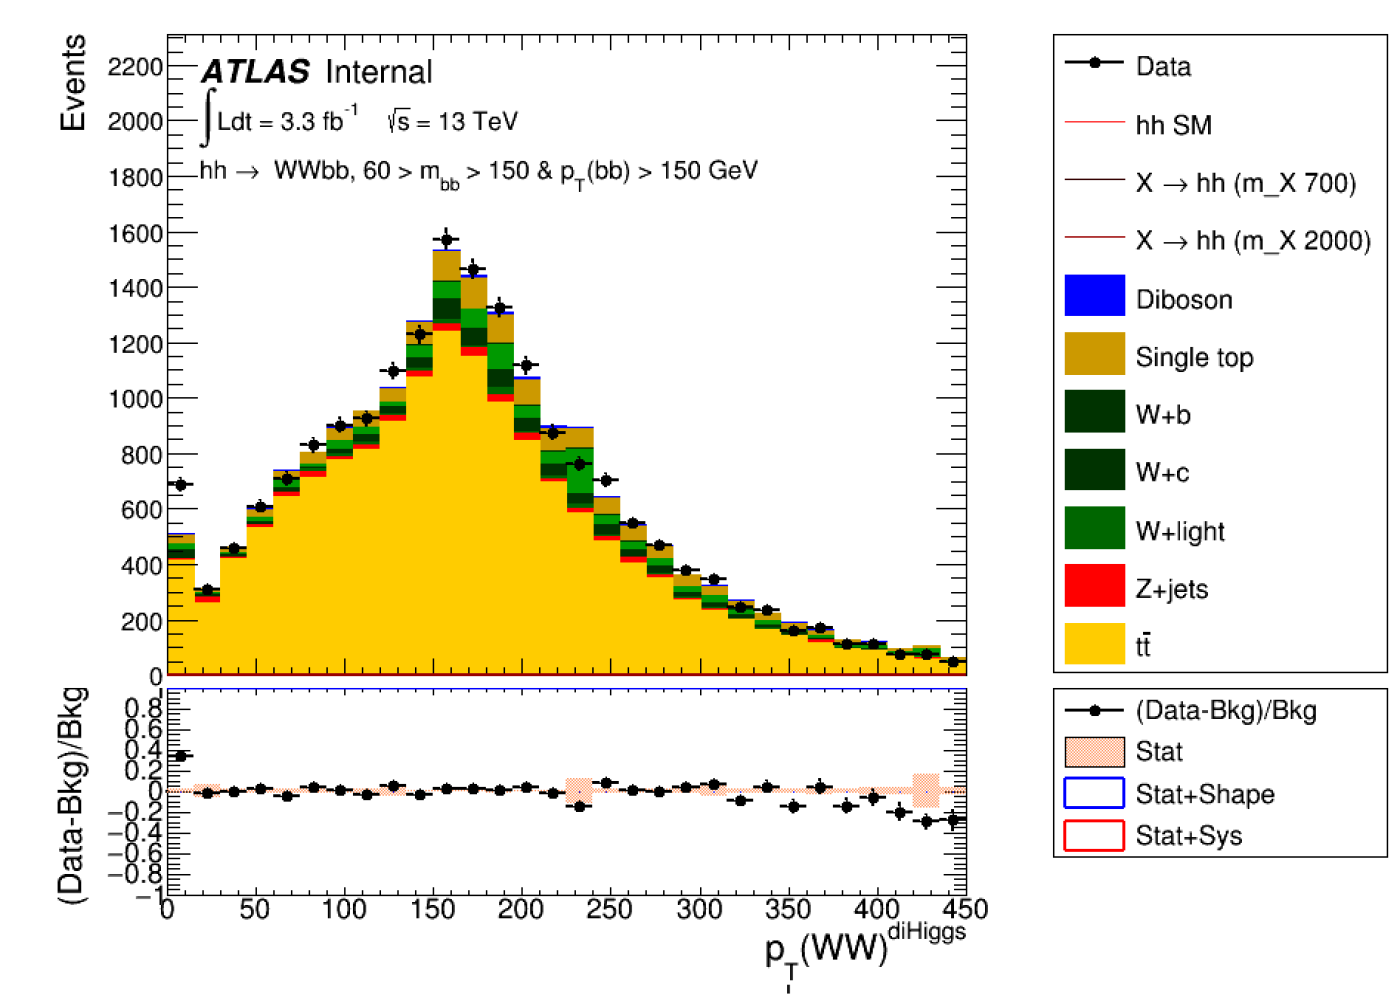
\includegraphics[width=.47\textwidth]{figures/kinFit_appendix/bbpt150_NF1168/C_mBBcr_opt700_bbpt150_KLF_dihiggs_ww_pt}
                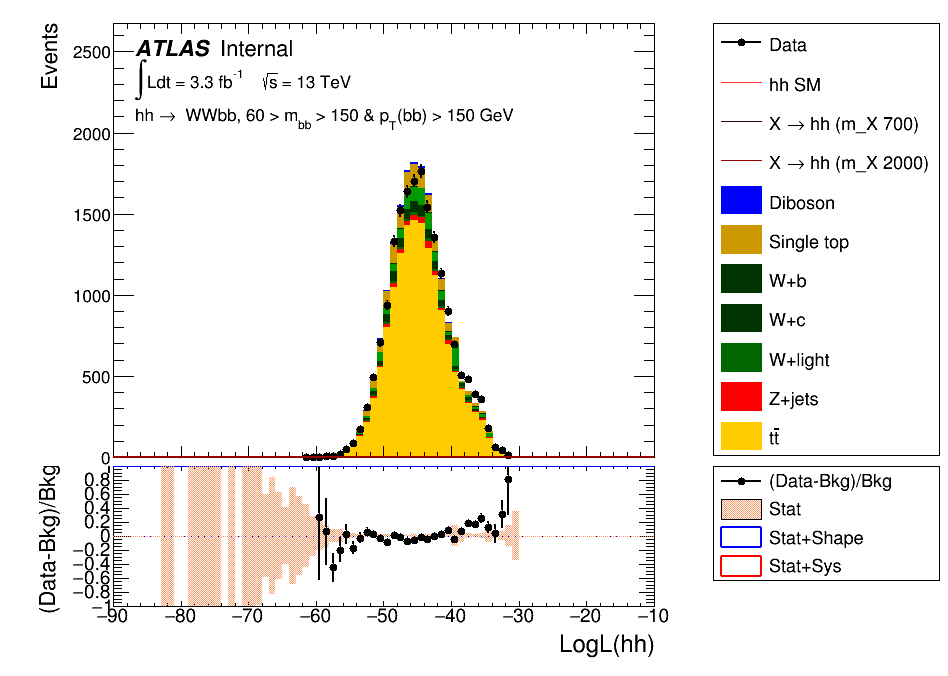
\includegraphics[width=.47\textwidth]{figures/kinFit_appendix/bbpt150_NF1168/C_mBBcr_opt700_bbpt150_LogLikelihood_dihiggs}
	\caption{These control plots show data/prediction agreement using the dihiggs kinematic fitting hypothesis in CR1 for select measured kinematics and the log likelihood of the leading permutation (ranked by event probability) after normalising $t\bar{t}$ as described in Sec~\ref{subsec:topCR}.}
	\label{fig:klfitter_control_plots_hh_bbpt150_nf1168}
	\end{center}    
	\end{figure}

\begin{figure}[!hb]
\begin{center}
		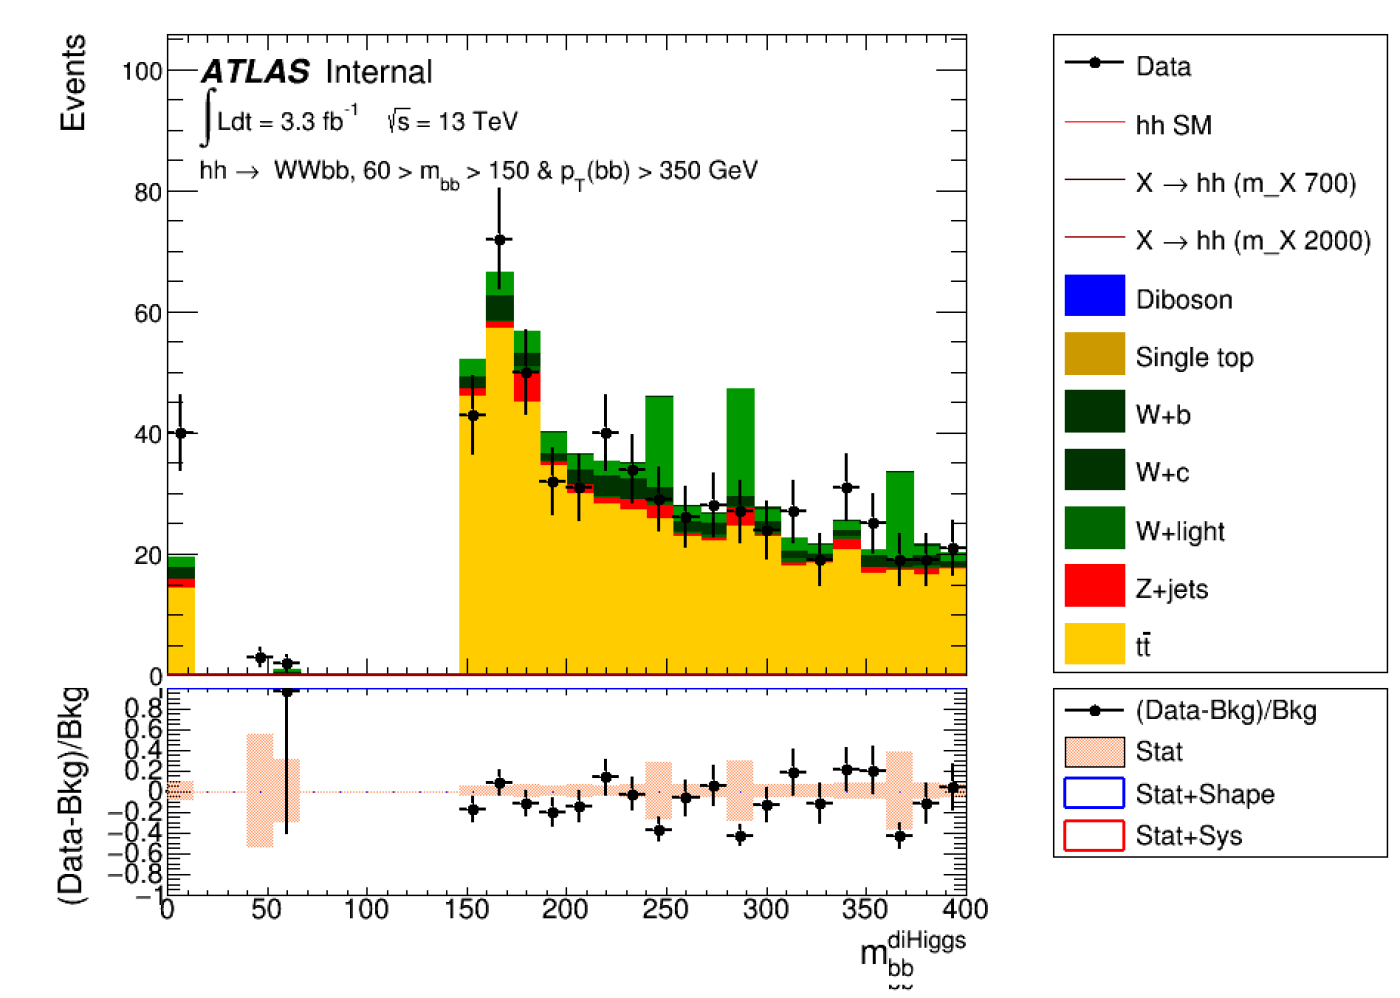
\includegraphics[width=.47\textwidth]{figures/kinFit_appendix/bbpt350_NF1190/C_mBBcr_opt2000_bbpt350_KLF_dihiggs_bb_m}
		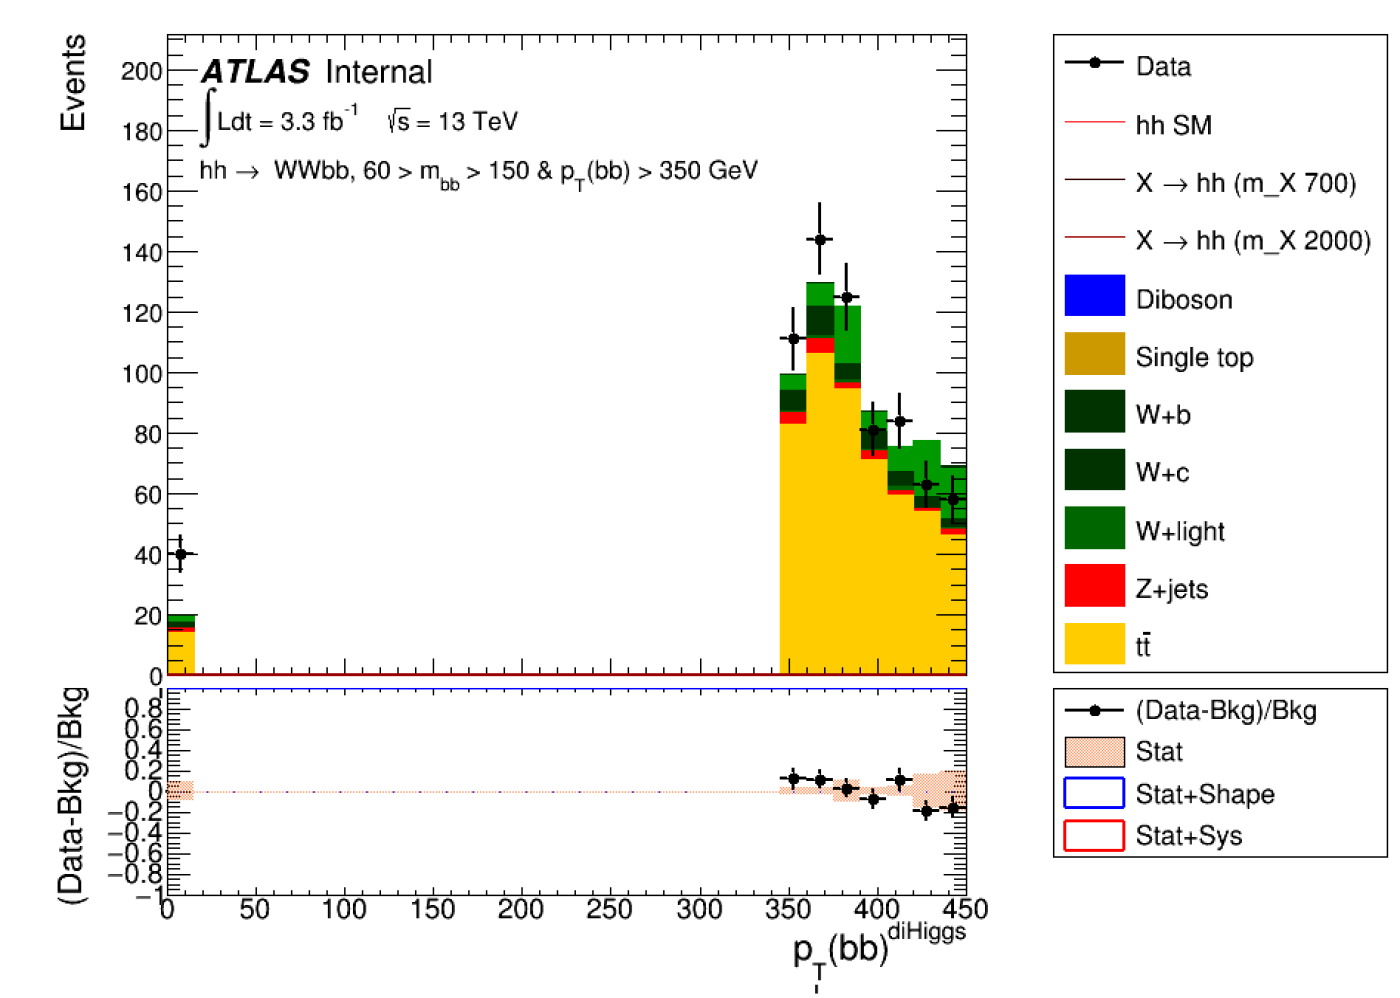
\includegraphics[width=.47\textwidth]{figures/kinFit_appendix/bbpt350_NF1190/C_mBBcr_opt2000_bbpt350_KLF_dihiggs_bb_pt}\\
		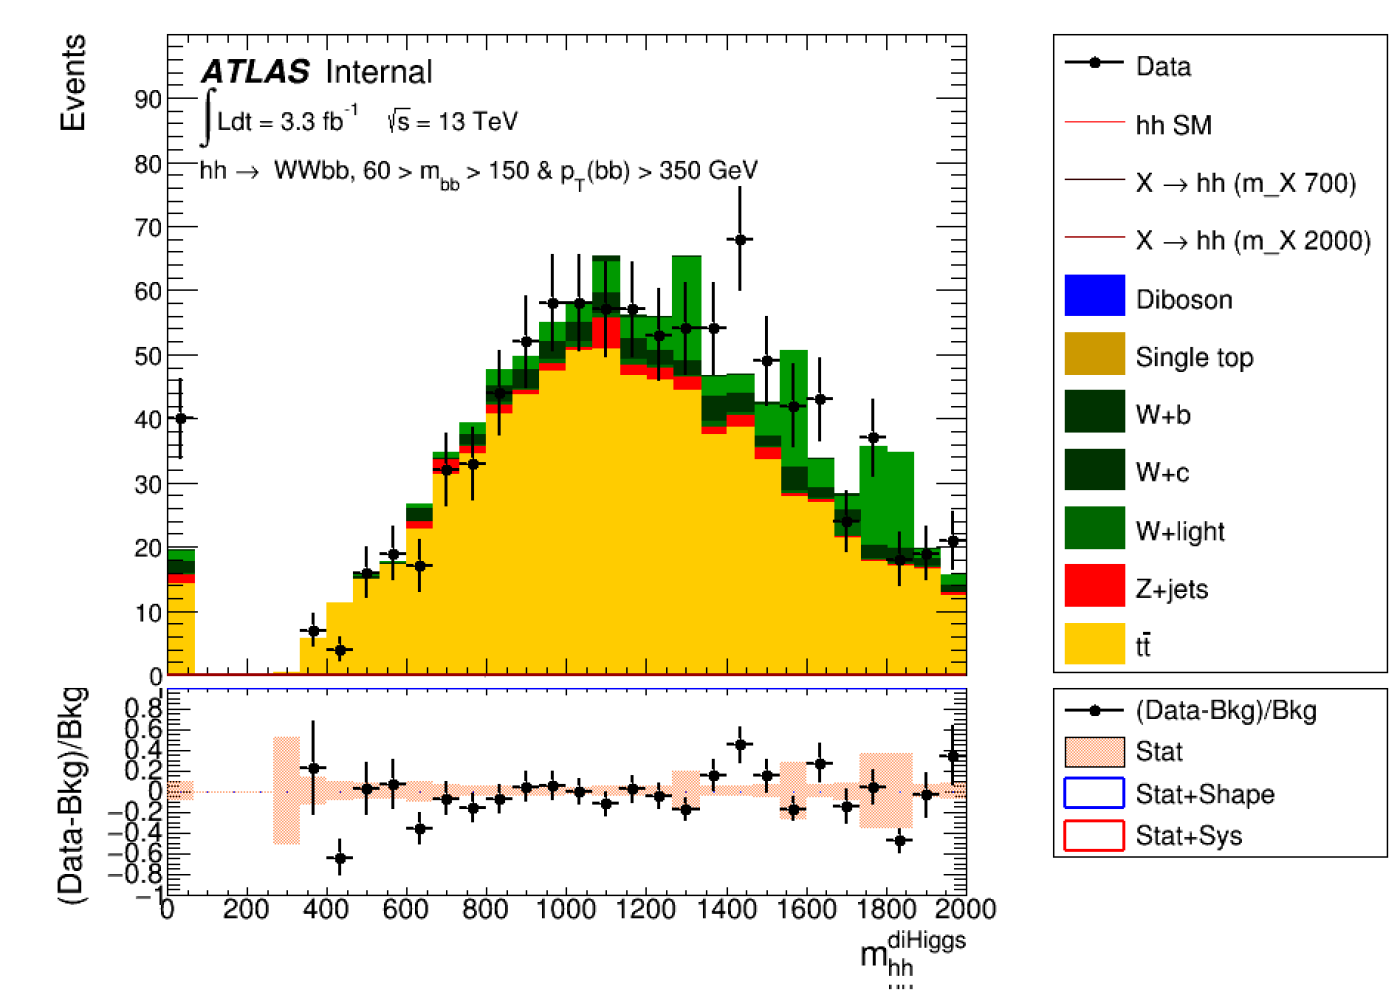
\includegraphics[width=.47\textwidth]{figures/kinFit_appendix/bbpt350_NF1190/C_mBBcr_opt2000_bbpt350_KLF_dihiggs_hh_m}
		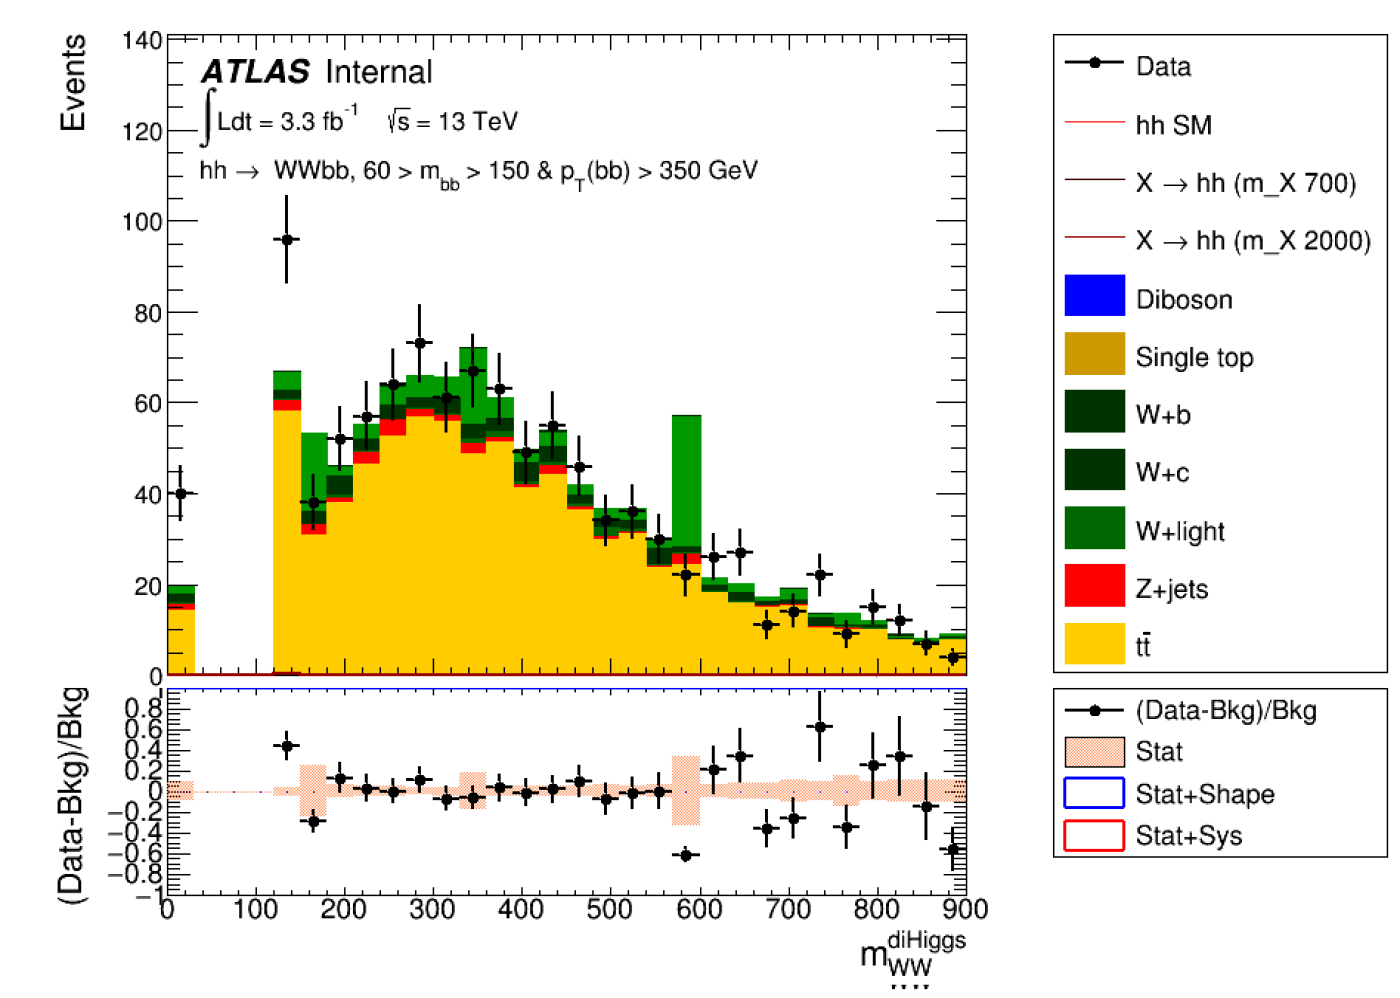
\includegraphics[width=.47\textwidth]{figures/kinFit_appendix/bbpt350_NF1190/C_mBBcr_opt2000_bbpt350_KLF_dihiggs_ww_m}\\
		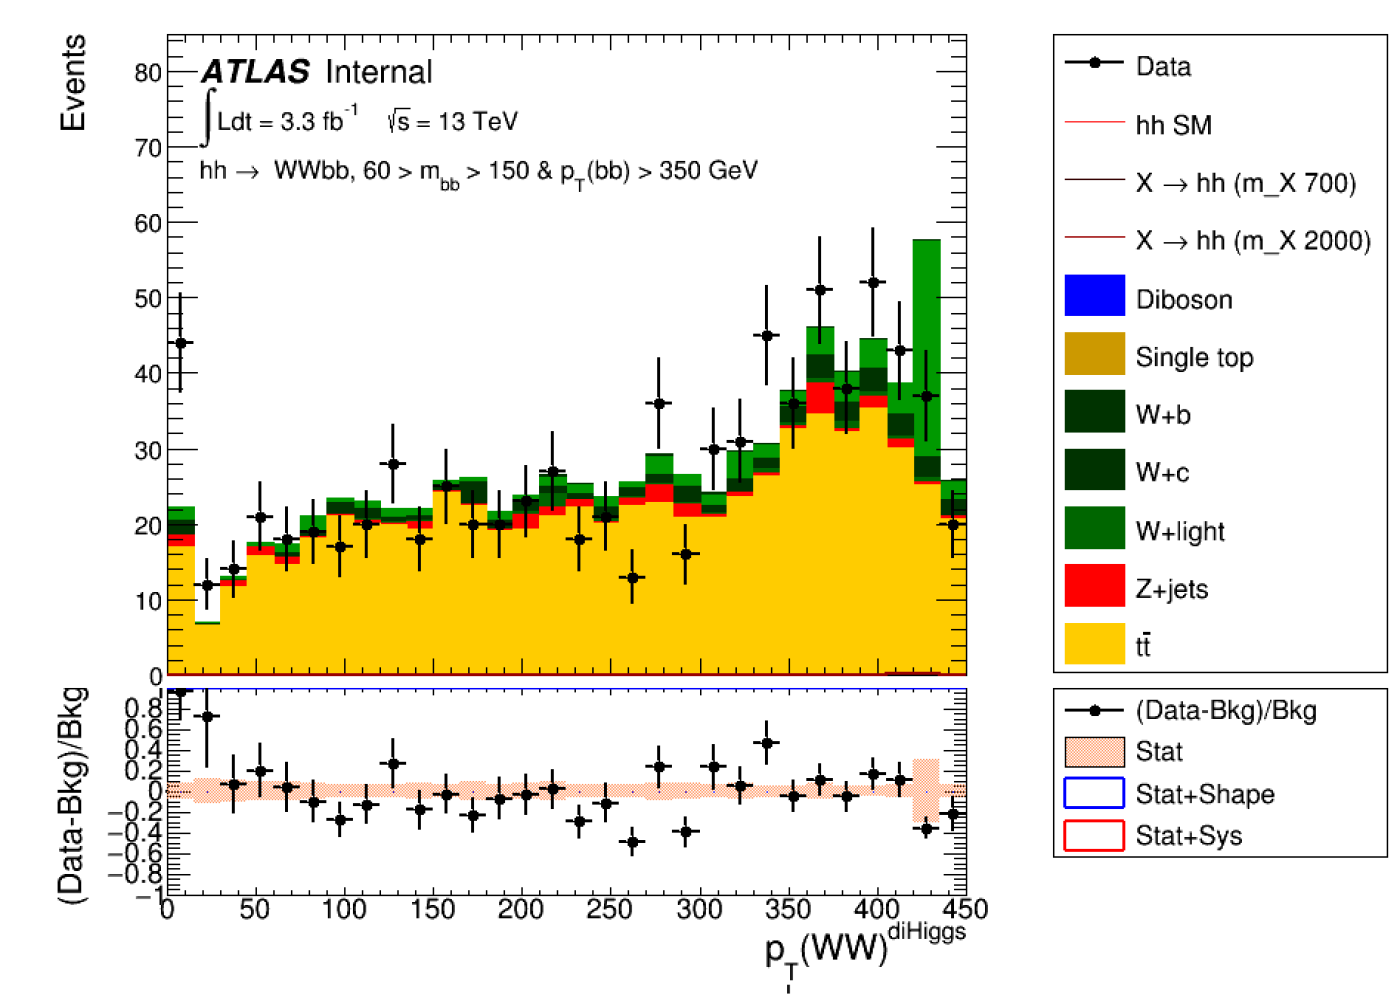
\includegraphics[width=.47\textwidth]{figures/kinFit_appendix/bbpt350_NF1190/C_mBBcr_opt2000_bbpt350_KLF_dihiggs_ww_pt}
                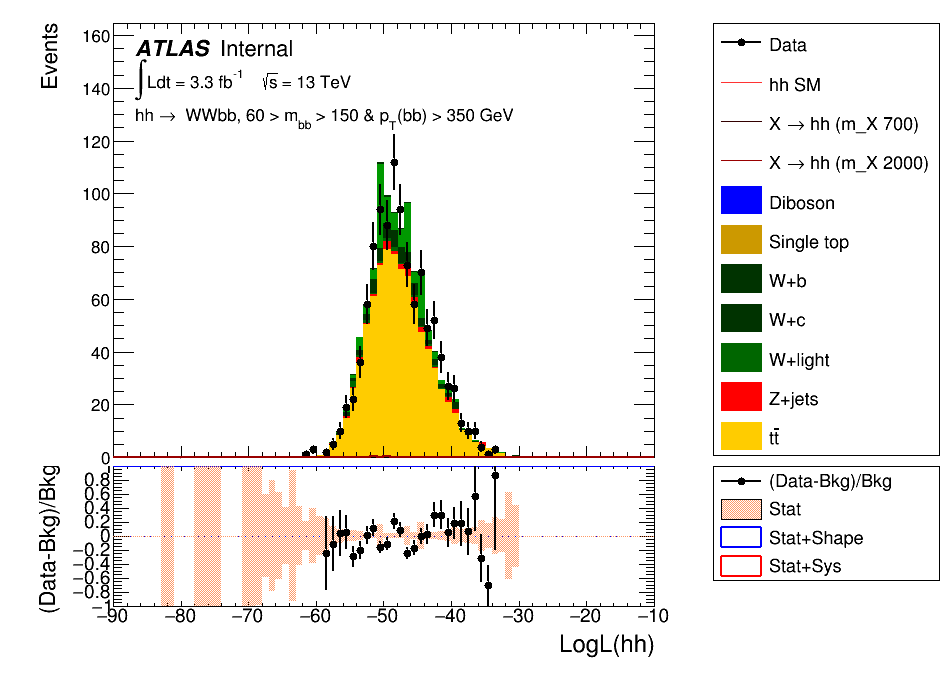
\includegraphics[width=.47\textwidth]{figures/kinFit_appendix/bbpt350_NF1190/C_mBBcr_opt2000_bbpt350_LogLikelihood_dihiggs}
	\caption{These control plots show data/prediction agreement using the dihiggs kinematic fitting hypothesis in CR1 for select measured kinematics and the log likelihood of the leading permutation (ranked by event probability) after normalising $t\bar{t}$ as described in Sec~\ref{subsec:topCR}.}
	\label{fig:klfitter_control_plots_hh_bbpt350_nf1190}
	\end{center}    
	\end{figure}


\subsubsection{KLFitter Optimization Study}
\label{sec:KLopt}
The efficiency of the kinematic fitting to correctly identify jet assignments relies on the jets available for permutation. As only the $t\bar{t}$ likelihood is used in the analysis, the KLFitter configuration was optimized using the $t\bar{t}$ Monte Carlo sample. Since each jet position is unique modulus the swapping of the light jets from $W$ decay (the $W$ mass constraint is invariant under a permutation of the two jets), supplying KLFitter with $n$ jets requires the likelihood calculation for a maximum $n!/2$ permutations. The number of permutations to be calculated is further reduced by rejecting permutations where non $b$ tagged jets are assigned to one of the jets expected to be one of the $b$ quarks. The optimal jet input configuration should maximize the matching efficiency of the reconstruction while balancing the CPU time required for each event. 
The matching efficiency is defined as
\begin{eqnarray}
\upepsilon_{\text{match}}=N_{\text{events}}^{\text{match}}/N_{\text{events}}^{\text{total}}
\label{eq:matchEff}
\end{eqnarray}
where $N_{\text{events}}^{\text{match}}$ can be defined in many ways (e.g. correctly matching all four jets, correctly matching only the $b$ jets, etc.). In the following discussion, an event is considered matched when all four reconstructed jets are correctly matched to their corresponding truth-level parton from the hard decay. Using these definitions, the final matching efficiencies are computed to find the optimal jet input configuration.

Many previous $t\bar{t}$ analyses use the four leading jets in $p_{T}$ as input to reconstruct the $t\bar{t}$ system. The simplest extension is increasing the number of input jets to five. In this case, the fitter will iterate through $5!=120$ permutations. Another option is to change the ordering by which jets are chosen to be included in the fit. In the 8 TeV ATLAS measurement of $t\bar{t}$ charge asymmetry \cite{Juste:1647184}, the two jets (taken from all jets passing object selection in the event) with the highest MV1 weights are selected, and then the remaining jets are re-ordered in $p_{T}$ and the three highest taken as input. 

For this analysis, three different input configurations are studied: four leading jets in $p_{T}$ (4-jet simple), five leading jets in $p_{T}$ (5-jet simple), two leading jets in MV1 + three highest $p_{T}$ jets remaining (5-jet advanced). The results are presented in Table \ref{tab:matchEff}.

\begin{table}[]
\centering
\begin{tabular}{l|l}
\hline \hline
Configuration  & $\ell$+jets \\ \hline
4-jet simple     &  0.260   \\
5-jet simple     &  0.292   \\
5-jet advanced   &  0.323   \\ \hline \hline
\end{tabular}
\caption{Matching efficiencies for different KLFitter input jet configurations. An event is considered matched if all four truth jets from the hard $t\bar{t}$ decay are bi-uniquely matched (within a $\Delta R\leq 0.3$) to four reconstructed jets of the leading KLFitter permutation.}
\label{tab:matchEff}
\end{table}

Since the 5-jet advanced configuration was found to have the highest efficiency and the computing time required was reasonable, it was chosen as the final configuration for the $t\bar{t}$ kinematic fitting.


